% Pandoc/Quarto template for den-paper extension
\documentclass[
  manuscript=article,
  layout=publish,
  year=2026,
  volume=1,
]{den}

% DOI

% Conference (for proceedings/poster)

% Dates
\published{22 Juli 2026}

% Editor and reviewers

% Strip abstract fields from bibliography entries (prevents LuaLaTeX parsing issues)

% Title
\title{Revitalisasi Industri Padat Karya Indonesia: Tekstil, Garmen, dan
Alas Kaki di Bawah Tekanan Rantai Nilai Global}

% Authors and affiliations
\author{Ahmad Nugroho}
\affiliation{Dewan Ekonomi Nasional}
\author{Annisa Tikahardinda}
\affiliation{Dewan Ekonomi Nasional}
\author{Artstein Dhimathera}
\affiliation{Dewan Ekonomi Nasional}
\author{Gaffari Ramadhan}
\affiliation{Dewan Ekonomi Nasional}
\author{Krisna Gupta \orcid{0000-0001-8695-0514}}
\affiliation{Dewan Ekonomi Nasional}
\email{krisna@dewanekonomi.go.id}
\author{Latasha Safira}
\affiliation{Dewan Ekonomi Nasional}
\author{Shobrina Arifin}
\affiliation{Dewan Ekonomi Nasional}
\author{Tiara Ariyanda}
\affiliation{Dewan Ekonomi Nasional}

% Keywords
\keywords{tekstil dan garmen; alas kaki; rantai nilai global; kebijakan
industri; Indonesia}

% JEL classification codes
\jel{F14, L67, O25}

% Abbreviations

% Pandoc/Quarto compatibility macros
\providecommand{\tightlist}{%
  \setlength{\itemsep}{0pt}\setlength{\parskip}{0pt}}
\providecommand{\citeproc}[2]{#1}
\providecommand{\citeproctext}{}

% Support for graphics
\RequirePackage{graphicx}

% Support for ding symbols (checkmarks, etc.)
\RequirePackage{pifont}

% Support for table column width calculations (required by Quarto-generated tables)
\RequirePackage{calc}

% Pandoc image handling - required for newer Pandoc/Quarto versions
% Constrains images to text width to prevent overflow
\makeatletter
\providecommand{\pandocbounded}[1]{%
  \sbox0{#1}%
  \ifdim\wd0>\linewidth
    \resizebox{\linewidth}{!}{#1}%
  \else
    #1%
  \fi
}
\makeatother

% CSL references support
\newlength{\cslhangindent}
\setlength{\cslhangindent}{1.5em}
\newlength{\csllabelwidth}
\setlength{\csllabelwidth}{3em}
\makeatletter
\newcommand{\CSLNoBibLabel}{\renewcommand{\@biblabel}[1]{}}
\makeatother
\newenvironment{CSLReferences}[2]
 {\begin{list}{}%
  {\setlength{\leftmargin}{0pt}
   \setlength{\itemindent}{0pt}
   \setlength{\itemsep}{#2\baselineskip}
   \setlength{\parsep}{0pt}
   \setlength{\topsep}{0pt}
   \setlength{\partopsep}{0pt}
   \ifodd #1
     \setlength{\leftmargin}{\cslhangindent}
     \setlength{\itemindent}{-\cslhangindent}
   \fi}
  \CSLNoBibLabel}
 {\end{list}}

% Header includes
\makeatletter
\@ifpackageloaded{caption}{}{\usepackage{caption}}
\AtBeginDocument{%
\ifdefined\contentsname
  \renewcommand*\contentsname{Daftar Isi}
\else
  \newcommand\contentsname{Daftar Isi}
\fi
\ifdefined\listfigurename
  \renewcommand*\listfigurename{Daftar Gambar}
\else
  \newcommand\listfigurename{Daftar Gambar}
\fi
\ifdefined\listtablename
  \renewcommand*\listtablename{Daftar Tabel}
\else
  \newcommand\listtablename{Daftar Tabel}
\fi
\ifdefined\figurename
  \renewcommand*\figurename{Gambar}
\else
  \newcommand\figurename{Gambar}
\fi
\ifdefined\tablename
  \renewcommand*\tablename{Tabel}
\else
  \newcommand\tablename{Tabel}
\fi
}
\@ifpackageloaded{float}{}{\usepackage{float}}
\floatstyle{ruled}
\@ifundefined{c@chapter}{\newfloat{codelisting}{h}{lop}}{\newfloat{codelisting}{h}{lop}[chapter]}
\floatname{codelisting}{Daftar}
\newcommand*\listoflistings{\listof{codelisting}{Daftar Daftar}}
\makeatother
\makeatletter
\makeatother
\makeatletter
\@ifpackageloaded{caption}{}{\usepackage{caption}}
\@ifpackageloaded{subcaption}{}{\usepackage{subcaption}}
\makeatother

% Keep internal links clickable without PDF border underlines.
\hypersetup{pdfborder={0 0 0}}

% Source note environment for figure attributions (right-aligned, compact)
% \FloatBarrier forces pending floats to appear before the note, so the
% figure and its source line always land on the same page.
\RequirePackage{placeins}
\newenvironment{source}{%
  \FloatBarrier%
  \vspace{-1em}%
  \begin{flushright}\scriptsize\itshape
}{%
  \end{flushright}%
}
\newcommand{\sumber}[1]{%
  \FloatBarrier%
  \vspace{-1em}%
  \begin{flushright}\scriptsize\itshape
  Sumber: #1
  \end{flushright}%
}

% Allow URLs in bibliography to break across lines at any character.
% \UrlOrds adds break opportunities after all ordinary characters so long
% URLs (DOIs, web links) do not overflow the right margin.
\makeatletter
\g@addto@macro{\UrlBreaks}{\UrlOrds}
\makeatother

% Allow LaTeX more flexibility in line breaking to prevent overflow
% (needed for Indonesian/non-English text on narrow B5 paper)
\tolerance=1000
\emergencystretch=1.5em

\begin{document}

\begin{abstract}
Makalah ini membahas perkembangan dan daya saing industri tekstil \&
garmen serta alas kaki Indonesia. Kedua industri ini merupakan sumber
penting lapangan kerja formal dan terintegrasi erat ke dalam jaringan
produksi global. Makalah ini meninjau perkembangan terkini pada
investasi, perdagangan, teknologi, dan kesiapan tenaga kerja, serta
membahas tantangan utama yang memengaruhi daya saing industri. Makalah
ini juga menyoroti bahwa industri tekstil dan alas kaki terdiri atas
perusahaan yang beragam, yang beroperasi dengan model bisnis berbeda dan
menghadapi kendala yang berbeda di sepanjang rantai nilai.
Perbedaan-perbedaan tersebut memiliki implikasi penting bagi perancangan
kebijakan yang ditujukan untuk mendukung daya saing industri dan
pertumbuhan lapangan kerja.
\end{abstract}

\section{Pendahuluan}\label{pendahuluan}

Penciptaan lapangan kerja formal masih menjadi salah satu tantangan
utama pembangunan ekonomi Indonesia. Data Badan Pusat Statistik (BPS)
menunjukkan bahwa meskipun tingkat pengangguran terbuka menurun dari
4,91 persen pada Agustus 2024 menjadi 4,85 persen pada Agustus 2025,
tenaga kerja informal terus tumbuh lebih cepat dibandingkan tenaga kerja
formal. Pada saat yang sama, proporsi pekerja penuh waktu menunjukkan
tren yang menurun dalam beberapa tahun terakhir (BPS 2025b; Lubis 2025).
Perkembangan tersebut menunjukkan bahwa kinerja pasar tenaga kerja perlu
dinilai tidak hanya dari jumlah lapangan kerja yang tercipta, tetapi
juga dari kualitas dan formalitas kesempatan kerja tersebut.

Dalam konteks ini, industri tekstil \& garmen, serta alas kaki menempati
posisi strategis dalam perekonomian Indonesia. Pada 2025, kedua industri
tersebut mempekerjakan lebih dari lima juta pekerja, setara dengan
sekitar seperempat tenaga kerja manufaktur formal Indonesia. Kontribusi
keduanya terhadap penyerapan tenaga kerja jauh lebih besar secara
proporsional dibandingkan kontribusinya terhadap output manufaktur, yang
mencerminkan sifat padat karya dari proses produksinya. Berdasarkan data
BPS, kedua industri juga menghasilkan lapangan kerja per unit investasi
yang jauh lebih banyak dibandingkan sebagian besar sektor manufaktur
lainnya. Akibatnya, perkembangan industri tekstil dan alas kaki memiliki
implikasi langsung terhadap penciptaan lapangan kerja formal, pendapatan
rumah tangga, dan inklusi ekonomi yang lebih luas.

Pada saat yang sama, kedua industri menghadapi serangkaian tantangan
yang kompleks. Dalam beberapa tahun terakhir, produsen tekstil dan alas
kaki terdampak oleh perlambatan permintaan global, persaingan
internasional yang semakin ketat, persyaratan keberlanjutan yang semakin
ketat di pasar ekspor utama, serta kebutuhan akan peningkatan teknologi
dan produktivitas yang berkelanjutan. Tekanan-tekanan tersebut tercermin
dari penutupan pabrik dan pemutusan hubungan kerja yang dilaporkan sejak
2023. Namun demikian, di tengah tantangan tersebut, kedua industri tetap
menarik investasi baru, terutama dari perusahaan yang terintegrasi ke
dalam rantai nilai global dan memasok merek internasional. Kontradiksi
yang tampak ini menunjukkan bahwa tantangan yang dihadapi sektor ini
tidak dapat dipahami semata-mata sebagai persoalan menurunnya daya
saing. Sebaliknya, tantangan tersebut mencerminkan proses transformasi
industri yang sedang berlangsung dan membentuk ulang industri tekstil
dan alas kaki Indonesia.

Makalah ini menelaah dinamika tersebut secara lebih rinci. Bagian 2
meninjau karakteristik industri tekstil dan alas kaki Indonesia,
termasuk struktur rantai nilai, pola investasi, keterkaitan perdagangan,
dan heterogenitas industrinya. Bagian 3 membahas isu-isu strategis utama
yang memengaruhi daya saing industri, mencakup perdagangan
internasional, persyaratan keberlanjutan dan ketertelusuran, modernisasi
teknologi, serta kesiapan tenaga kerja. Bagian 4 meninjau kebijakan
pemerintah dan program dukungan yang relevan bagi pengembangan sektor
ini. Bagian 5 menutup makalah.

\section{Karakteristik Industri Tekstil \& Garmen dan Alas
Kaki}\label{karakteristik-industri-tekstil-garmen-dan-alas-kaki}

\subsection{Gambaran Umum}\label{gambaran-umum}

Gambar~\ref{fig-growth} menunjukkan pertumbuhan nilai tambah triwulanan
industri tekstil dan garmen serta industri kulit dan alas kaki,
dibandingkan dengan manufaktur nonmigas dan pertumbuhan ekonomi secara
umum. Industri tekstil dan garmen Indonesia tumbuh sebesar 3,55\% pada
2025, dibandingkan 4,26\% pada 2024. Industri kulit, barang dari kulit
dan alas kaki mencatat pertumbuhan sebesar 3,31 persen pada 2025,
setelah ekspansi yang jauh lebih kuat sebesar 6,83 persen pada 2024.
Meskipun terjadi moderasi pada 2025, industri alas kaki secara umum
berkinerja lebih baik dibandingkan industri tekstil selama periode
pemulihan pascapandemi. Secara lebih luas, kedua industri menunjukkan
volatilitas yang signifikan selama satu dekade terakhir, yang
mencerminkan pergeseran permintaan global dan disrupsi akibat pandemi
COVID-19.

\begin{figure}[htbp!]

\centering{

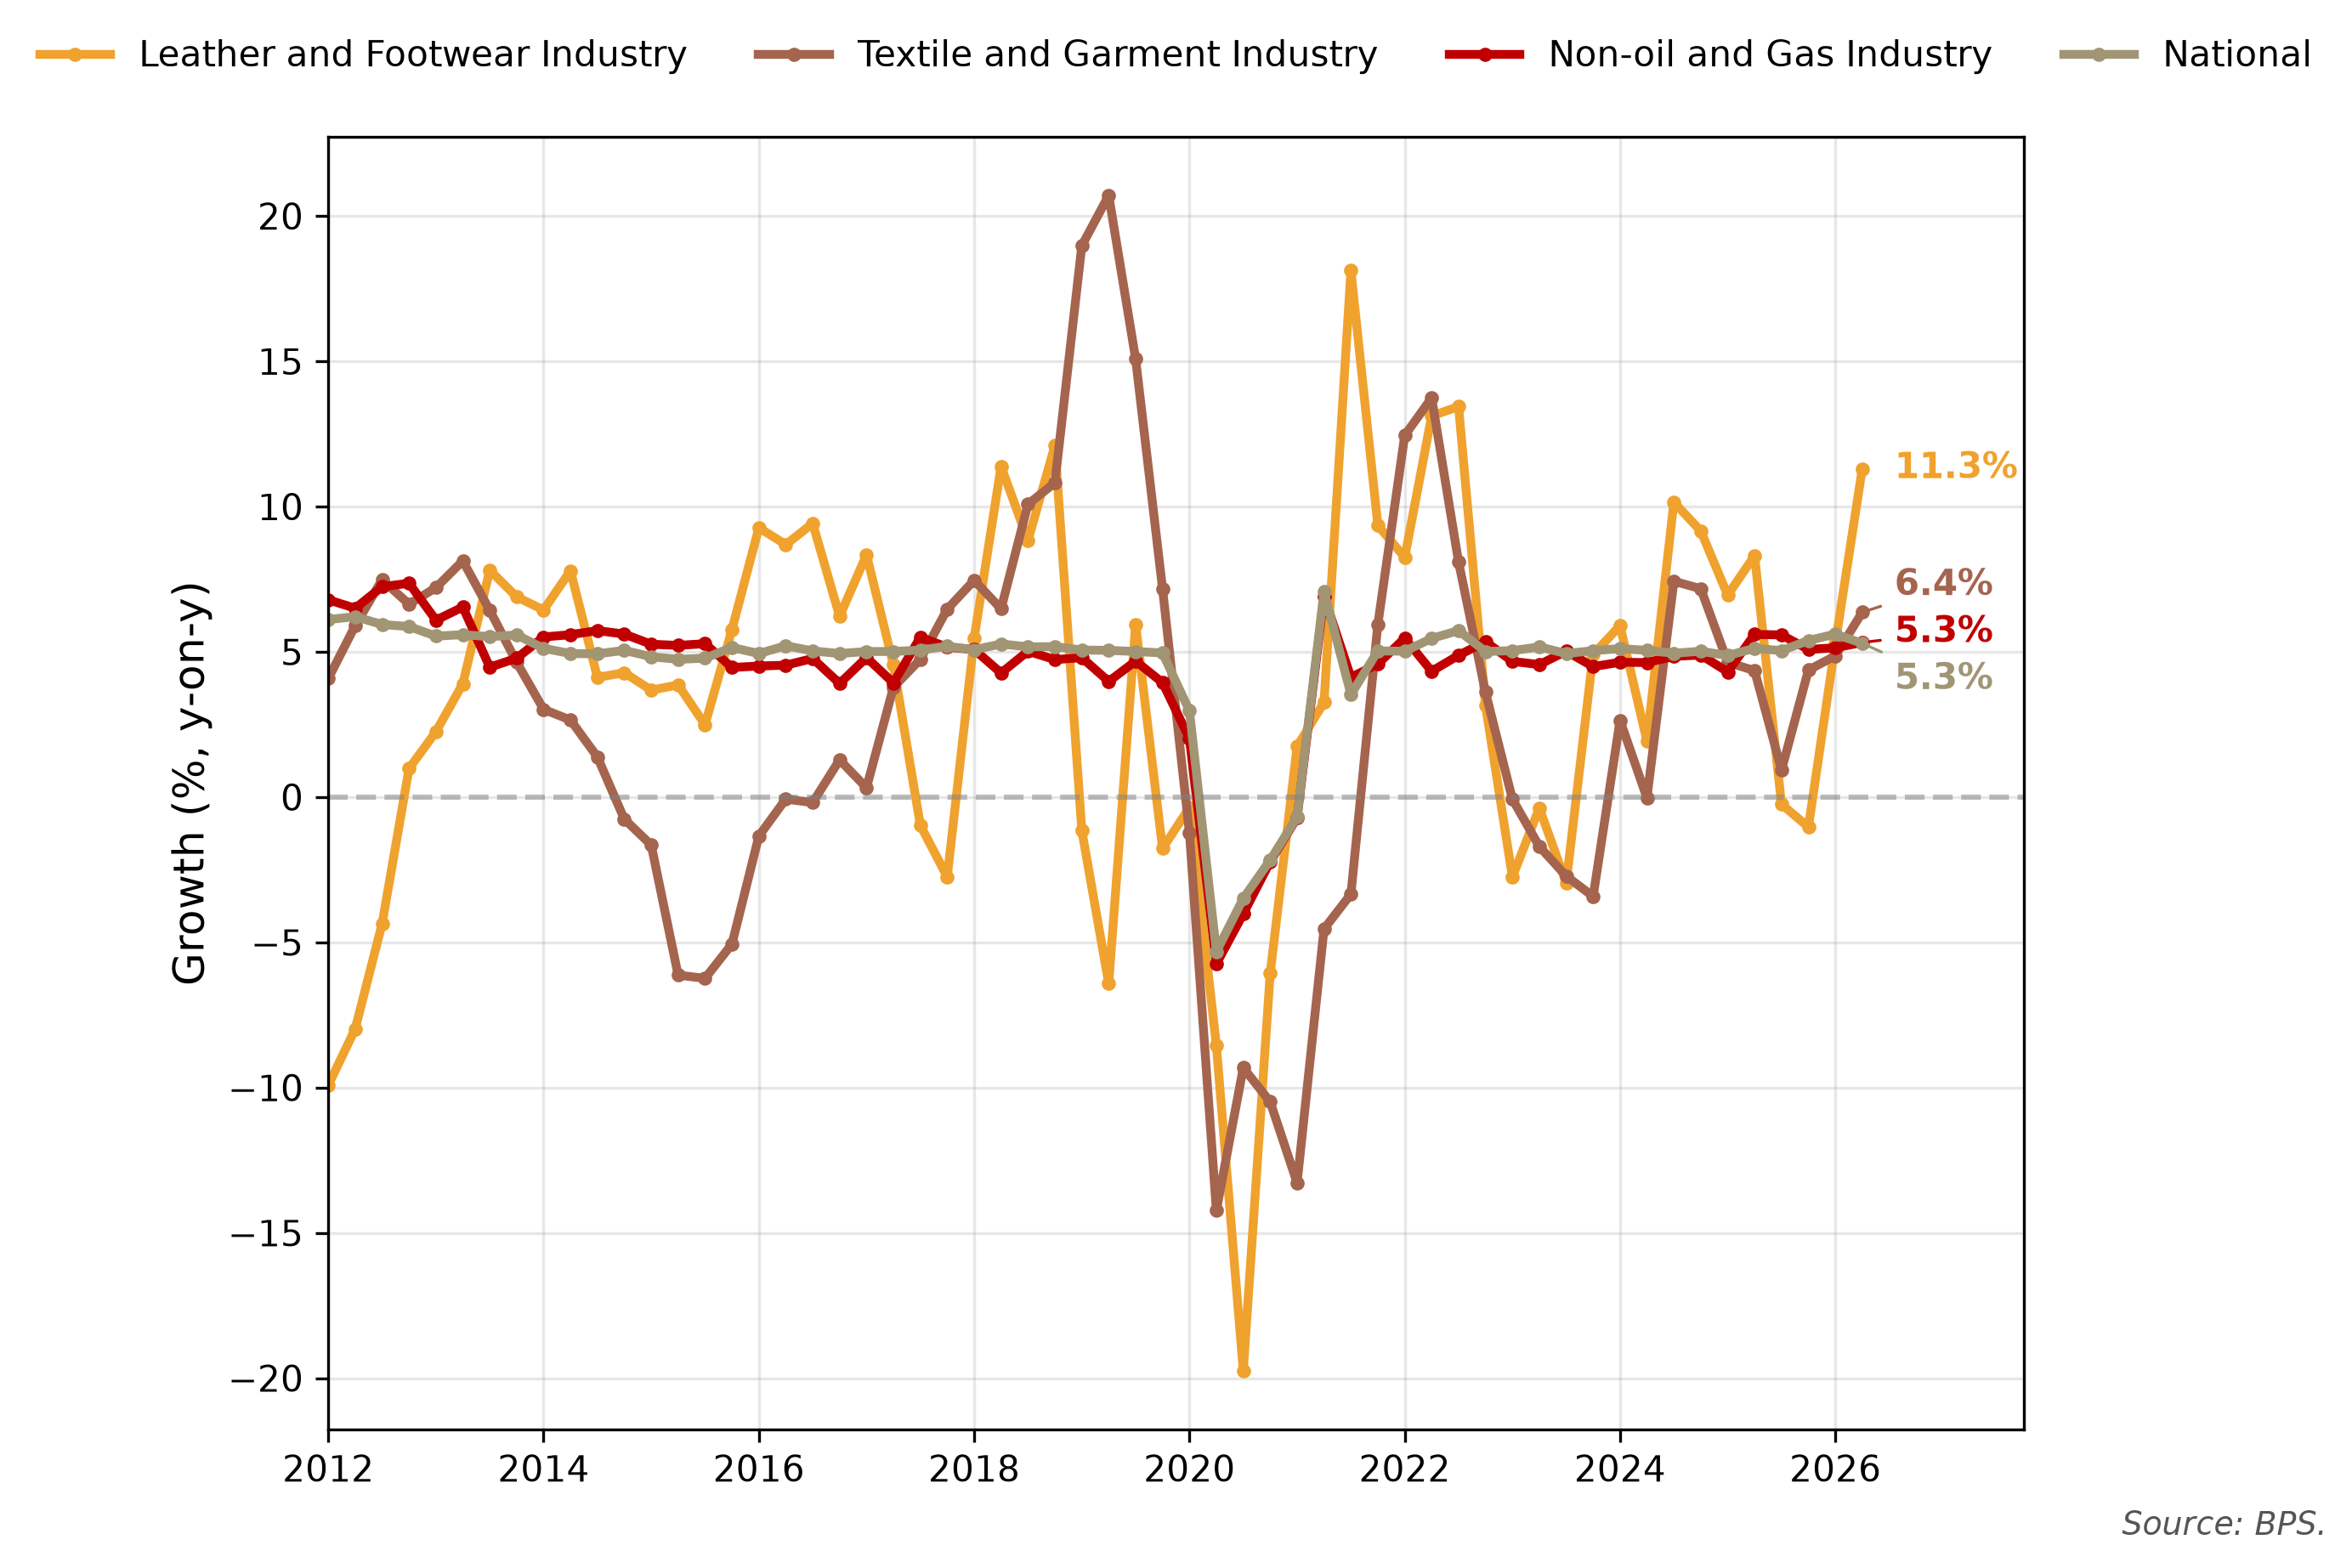
\includegraphics[width=0.85\linewidth,height=\textheight,keepaspectratio]{fig/gdp_growth_quarterly.png}

}

\caption{\label{fig-growth}Tren pertumbuhan sektor tekstil, alas kaki
dan manufaktur, 2010--2025. Sumber: BPS.}

\end{figure}%

Seperti ditunjukkan Gambar~\ref{fig-recovery}, lebih dari empat tahun
setelah pandemi bermula, kedua industri mengalami kondisi yang cukup
berbeda. Gambar tersebut menyajikan PDB harga konstan untuk industri
tekstil \& garmen dan industri alas kaki. Garis oranye solid menunjukkan
data PDB aktual, sedangkan garis putus-putus menunjukkan tren prapandemi
COVID yang diestimasi menggunakan metode filter HP (Hodrick dan Prescott
1997; Razzak 1997). Industri alas kaki tampak mampu kembali ke jalur
pertumbuhan jangka panjangnya. Industri tekstil dan garmen, sebaliknya,
masih kesulitan mengejar lintasan prapandemi COVID-nya.

\begin{figure}[htbp!]

\centering{

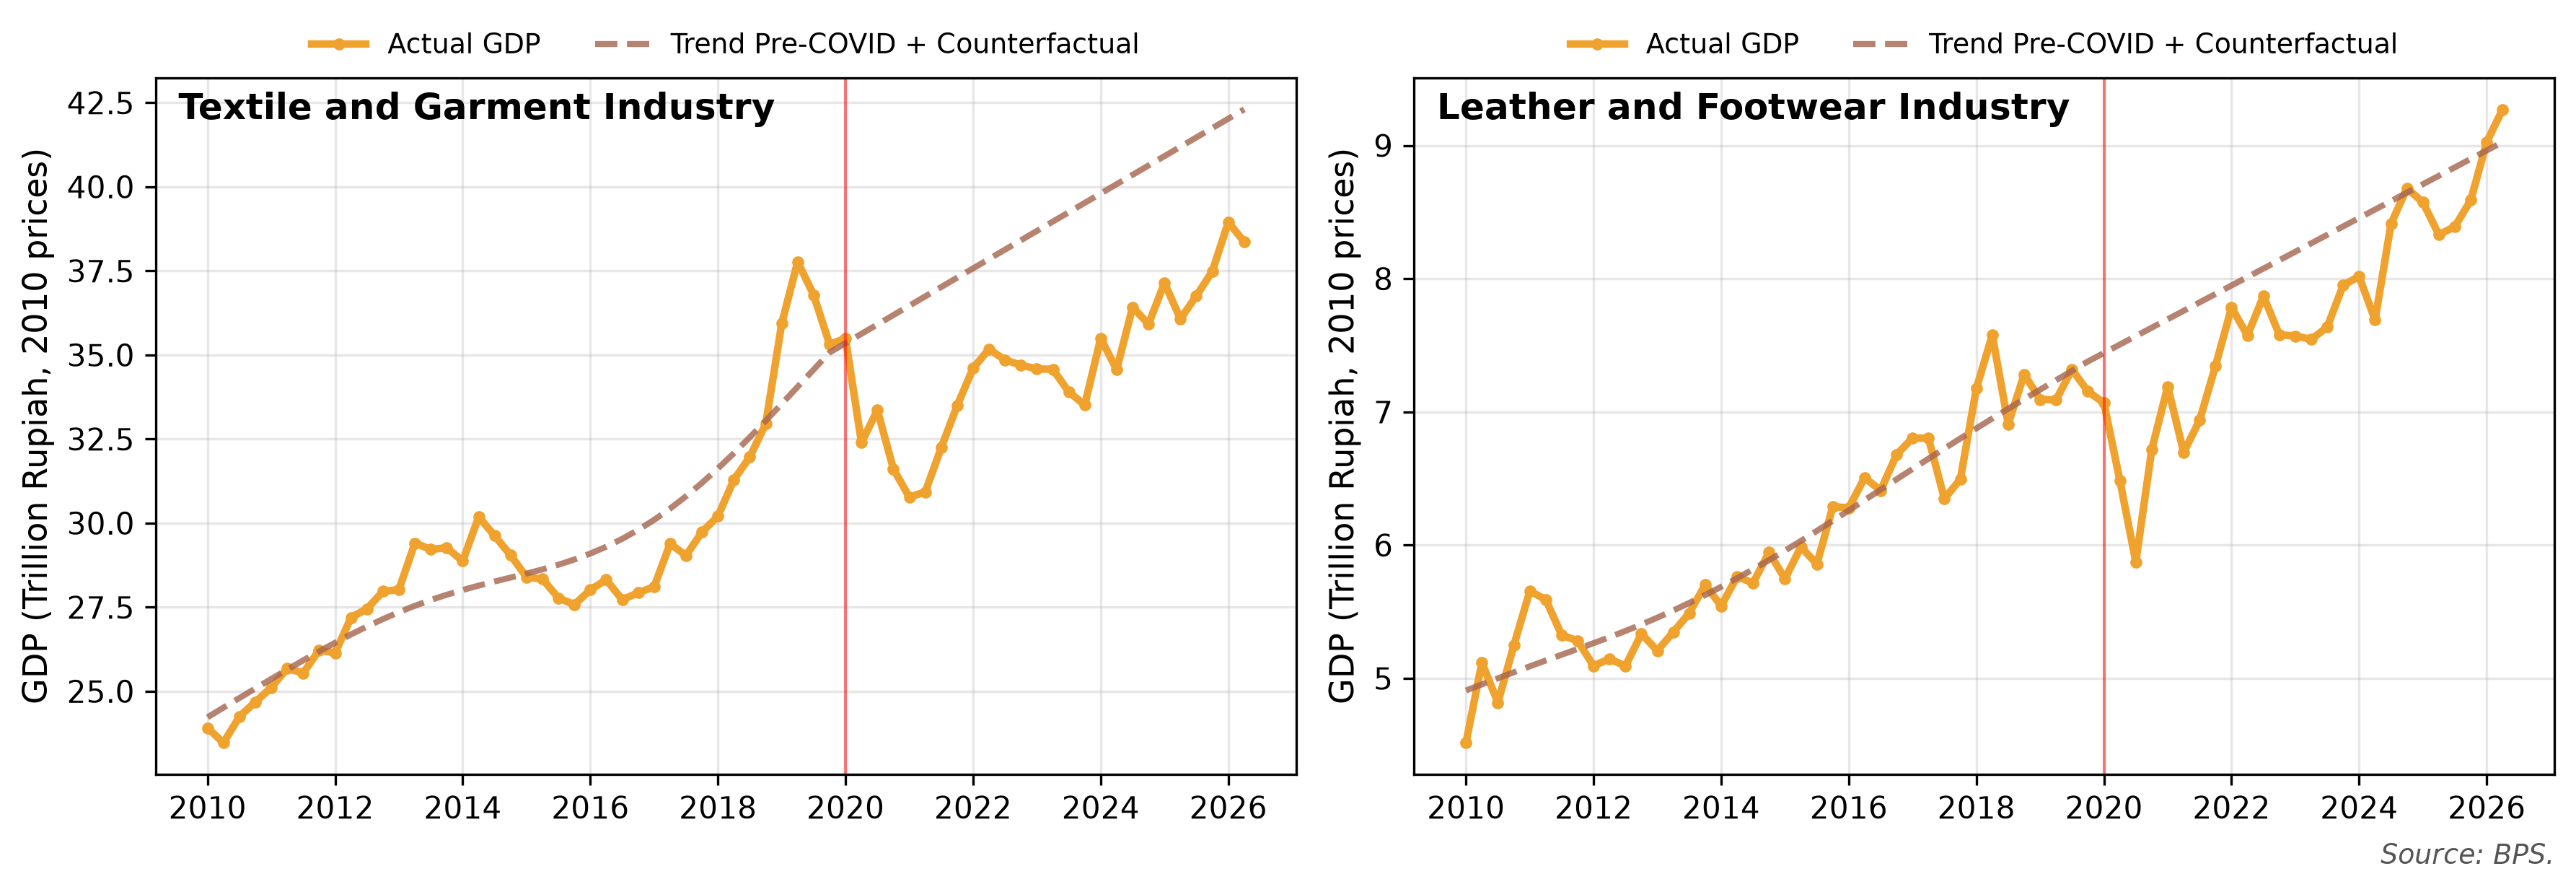
\includegraphics[width=1\linewidth,height=\textheight,keepaspectratio]{fig/gdp_covid_disruption_quarterly.png}

}

\caption{\label{fig-recovery}Proyeksi pemulihan pascapandemi industri
tekstil dan alas kaki relatif terhadap tren prapandemi COVID. Sumber:
BPS}

\end{figure}%

Investasi langsung pada kedua industri meningkat secara substansial
sejak pandemi COVID-19, mencapai level tertingginya selama 2021--2025
(Gambar~\ref{fig-investment}). Namun, kedua industri menunjukkan
struktur investasi yang sangat berbeda. Industri tekstil dan garmen
memiliki basis investasi yang relatif lebih luas, dengan investor
domestik menyumbang antara 19 hingga 61 persen dari total realisasi
investasi selama 2010--2025. Sebaliknya, industri alas kaki tetap sangat
bergantung pada penanaman modal asing (PMA), dengan investor asing
secara konsisten menyumbang sekitar 90 persen atau lebih dari total
investasi sepanjang sebagian besar periode tersebut.

\begin{figure}[htbp!]

\centering{

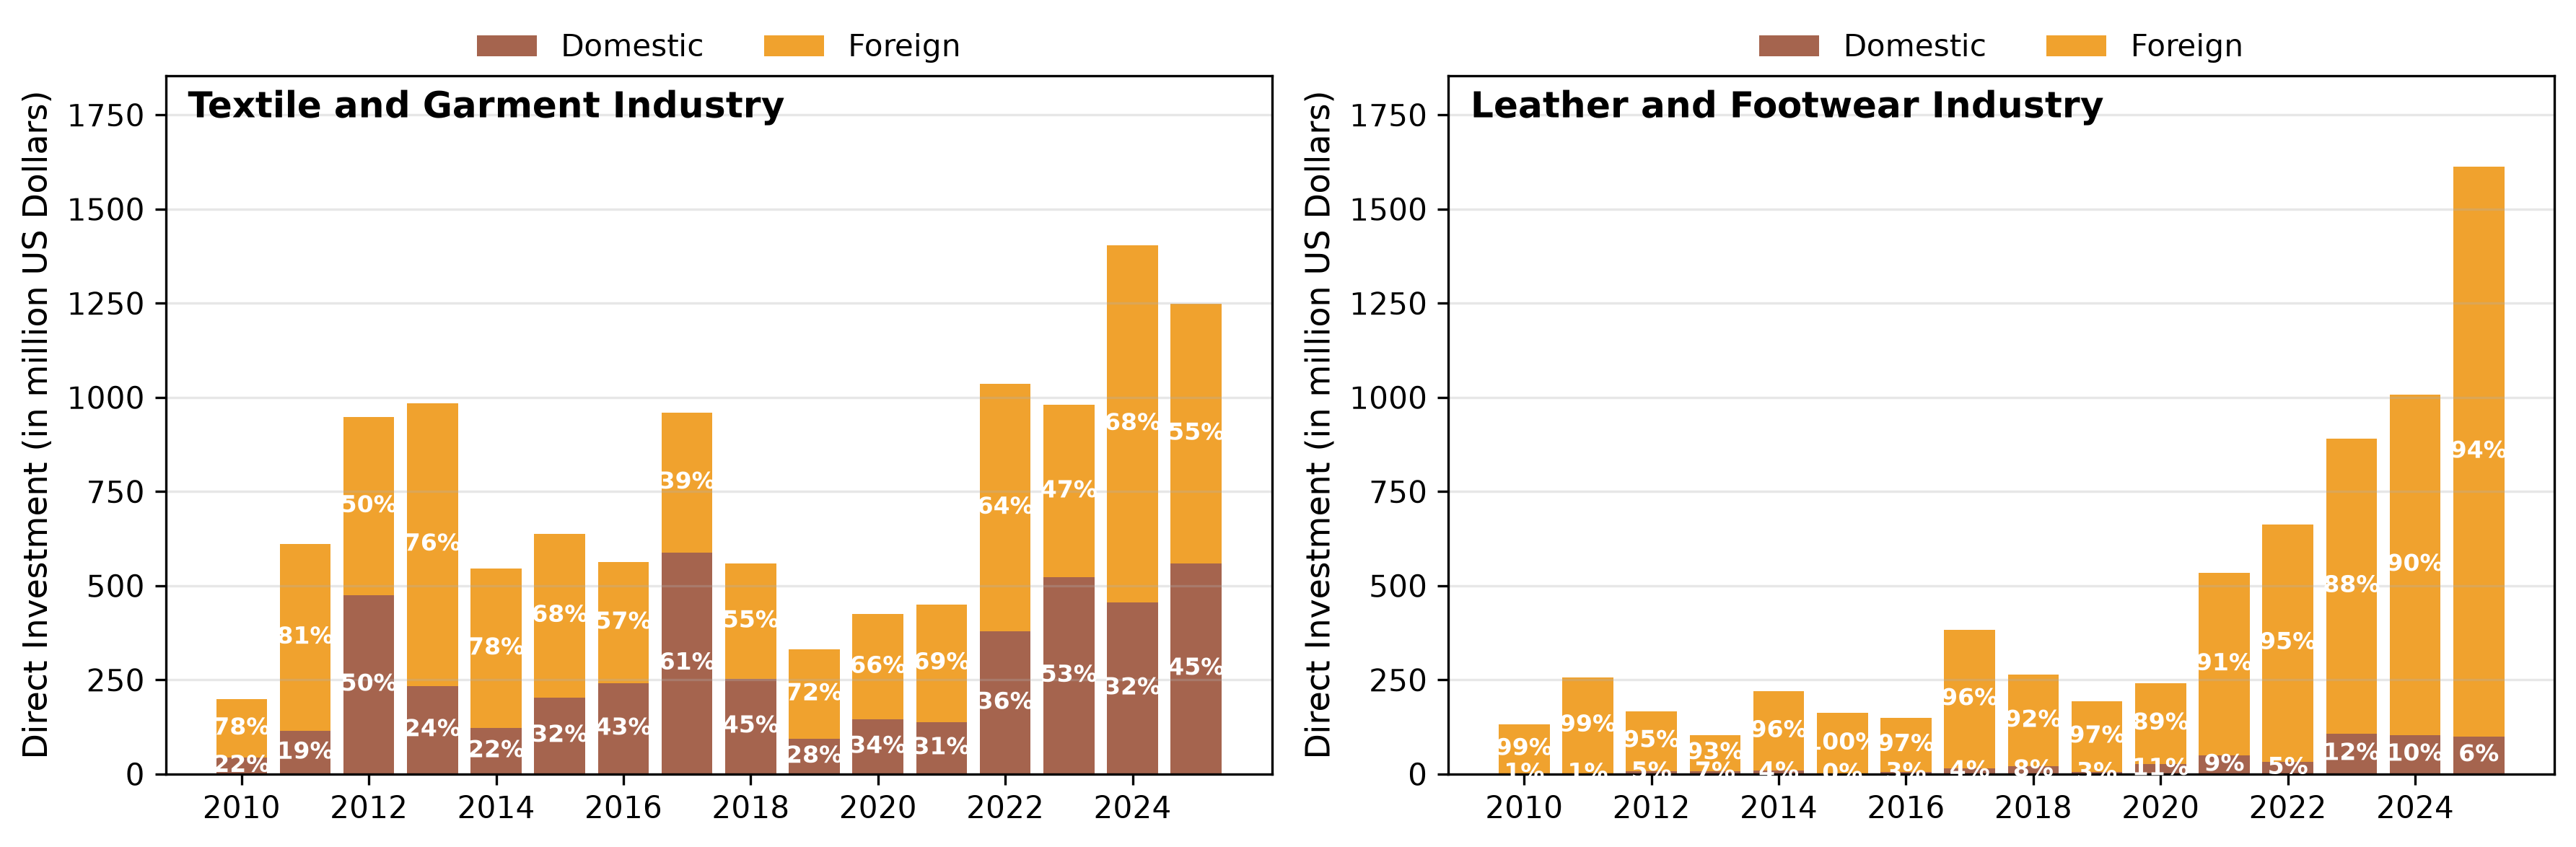
\includegraphics[width=1\linewidth,height=\textheight,keepaspectratio]{fig/investment_comparison.png}

}

\caption{\label{fig-investment}Investasi langsung asing dan domestik
pada industri tekstil dan alas kaki, 2010--2025. Sumber: BPS, diakses
melalui CEIC.}

\end{figure}%

Pertumbuhan investasi terutama menonjol pada industri alas kaki. Antara
2020 dan 2025, total realisasi investasi meningkat dari sekitar USD 241
juta menjadi lebih dari USD 1,6 miliar. Pada periode yang sama,
investasi pada industri tekstil dan garmen naik dari sekitar USD 424
juta menjadi USD 1,25 miliar. Akibatnya, pada 2025 industri alas kaki
menarik investasi yang lebih tinggi dibandingkan industri tekstil dan
garmen meskipun ukurannya jauh lebih kecil dari sisi output. Dominasi
investasi asing pada industri alas kaki konsisten dengan partisipasinya
yang kuat dalam jaringan produksi berorientasi ekspor, sementara
industri tekstil dan garmen terus memperoleh manfaat dari bauran
investasi domestik dan asing yang lebih terdiversifikasi.

Pentingnya kedua industri ini juga tercermin dari kinerja ekspornya.
Pada 2025, industri tekstil dan garmen Indonesia mencatat nilai ekspor
sebesar USD 11,98 miliar dan menghasilkan surplus perdagangan sebesar
USD 2,81 miliar. Nilai ekspor menurun tipis sebesar 0,6 persen (yoy),
dibandingkan pertumbuhan 3,1 persen pada 2024.

Sebaliknya, industri alas kaki terus mencatat kinerja ekspor yang kuat.
Ekspor alas kaki mencapai USD 7,98 miliar pada 2025, meningkat 9,54
persen (yoy), dibandingkan pertumbuhan 13,13 persen pada 2024. Dengan
impor sekitar USD 1,32 miliar, industri ini mempertahankan surplus
perdagangan yang substansial. Angka-angka tersebut menegaskan pentingnya
kedua industri sebagai sumber penerimaan ekspor, sekaligus menyoroti
momentum ekspor yang lebih kuat yang saat ini teramati pada industri
alas kaki.

Perdagangan internasional memainkan peran yang sangat penting baik pada
industri tekstil maupun alas kaki. Dengan menggunakan Tabel Input-Output
Multi-Regional (MRIO) Asian Development Bank (Asian Development Bank
2025), dapat diestimasi bahwa sekitar 41,88 persen output industri
tekstil pada akhirnya dialokasikan ke pasar ekspor, sementara angka yang
sama untuk industri alas kaki mencapai 92,81 persen. Input impor juga
tetap menjadi komponen produksi yang kritis. Berdasarkan estimasi yang
diturunkan dari kerangka MRIO yang sama, nilai barang dan jasa yang
bersumber dari luar negeri mencakup sekitar 72,88 persen dari total
input antara yang digunakan industri tekstil dan 84,23 persen pada
industri alas kaki. Angka-angka tersebut menunjukkan sejauh mana kedua
industri terintegrasi ke dalam jaringan produksi regional dan global,
baik sebagai eksportir maupun sebagai pengguna input yang bersumber dari
luar negeri.

Amerika Serikat dan Uni Eropa tetap menjadi dua pasar terpenting bagi
barang jadi tekstil dan alas kaki dunia. Keduanya secara bersama-sama
mencakup sekitar 64,2 persen impor global produk pada Bab HS 61--64 pada
2025, yang terutama terdiri atas pakaian jadi, barang tekstil jadi, dan
alas kaki (Gambar~\ref{fig-globalimport}). Uni Eropa merupakan importir
terbesar dunia untuk produk-produk tersebut, dengan pangsa 47,1 persen
dari total impor global, diikuti Amerika Serikat sebesar 17,1 persen.

\begin{figure}[htbp!]

\centering{

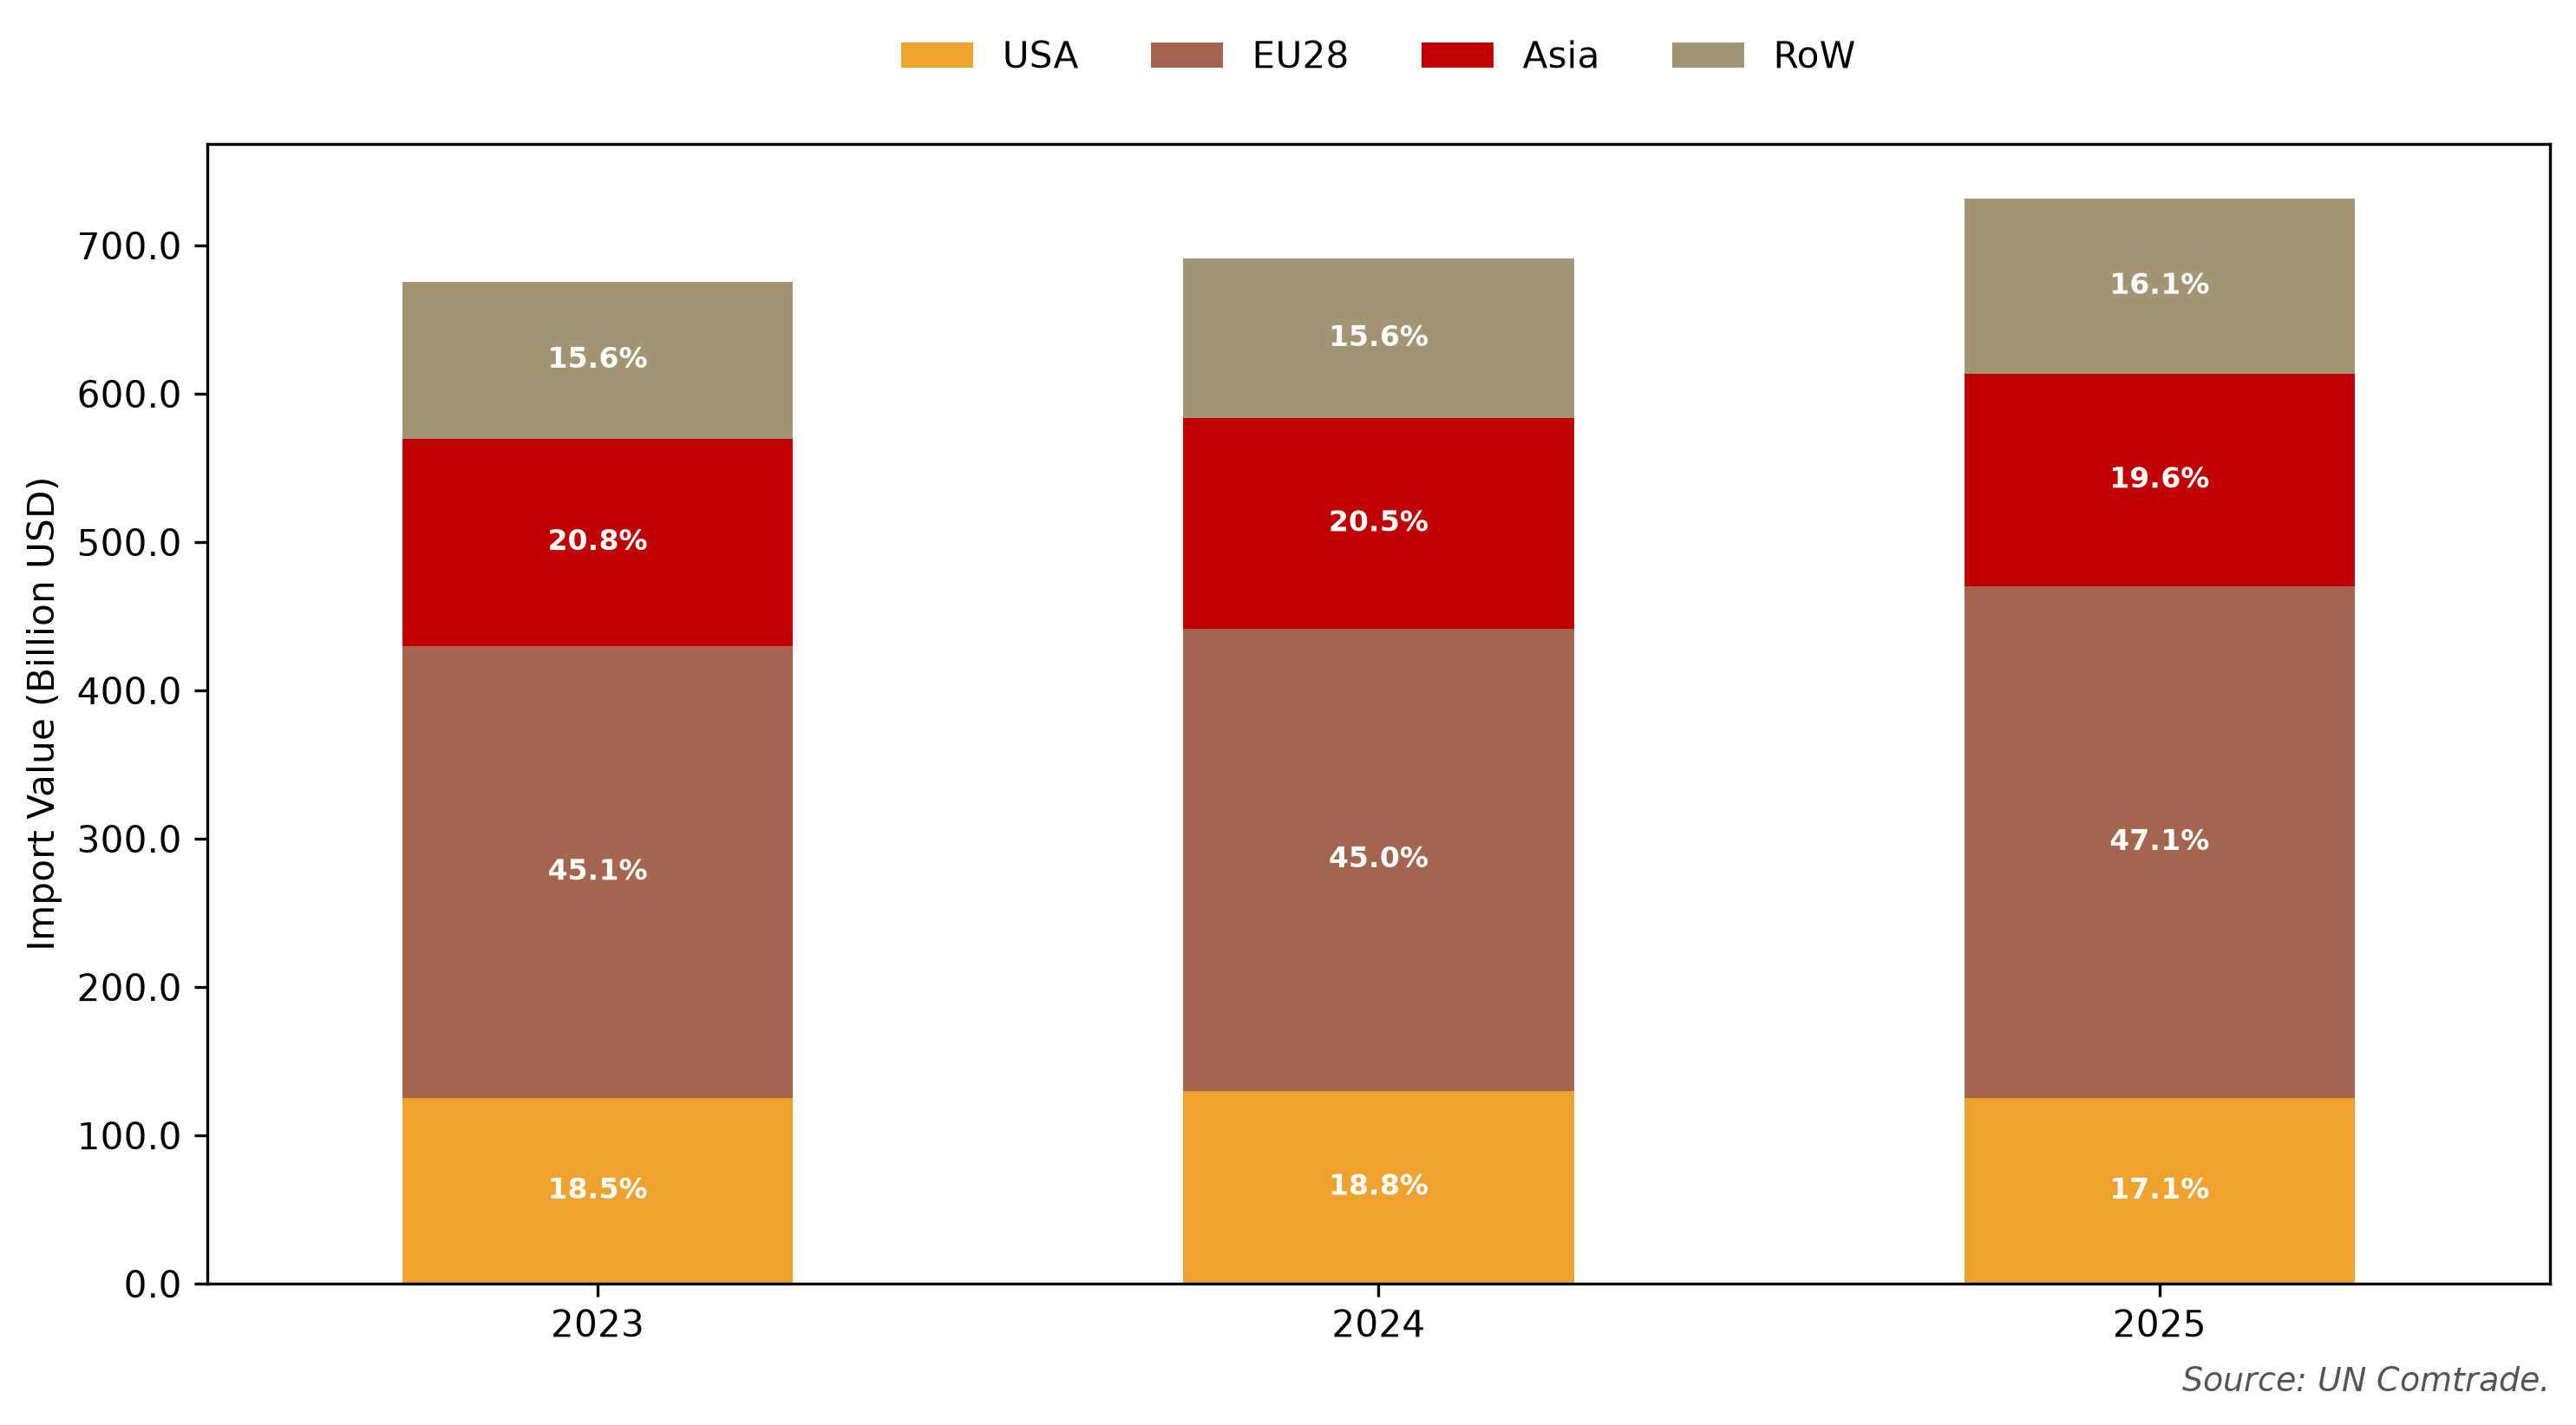
\includegraphics[width=0.85\linewidth,height=\textheight,keepaspectratio]{fig/fig1.png}

}

\caption{\label{fig-globalimport}Pasar impor global untuk garmen dan
alas kaki menurut kawasan, 2023--2025 (AS, UE, Asia dan Negara Lainnya
(RoW)). Sumbu y menunjukkan total nilai impor dalam miliar USD; label
menunjukkan pangsa masing-masing kawasan terhadap impor global. Sumber:
UN Comtrade.}

\end{figure}%

Selain perannya sebagai pasar ekspor utama, Uni Eropa juga berperan
penting dalam membentuk standar produksi global melalui inisiatif
regulasi seperti Ecodesign for Sustainable Products Regulation (ESPR)
(European Commission 2024; Yan 2025). Akibatnya, persyaratan
keberlanjutan dan ketertelusuran menjadi semakin penting bagi eksportir
tekstil dan alas kaki Indonesia yang ingin mengakses pasar Eropa.

Tabel~\ref{tbl-shares} menggambarkan bagaimana persaingan di pasar
ekspor tersebut berkembang selama satu dekade terakhir. Antara 2015 dan
2024, pangsa Tiongkok pada impor tekstil dan alas kaki menurun secara
substansial baik di Amerika Serikat maupun Uni Eropa. Di Amerika
Serikat, pangsa pasar Tiongkok turun dari 44,00\% menjadi 29,22\%,
sedangkan di Uni Eropa turun dari 39,09\% menjadi 30,70\%. Penerima
manfaat terbesar dari pergeseran ini adalah Vietnam dan Bangladesh, yang
keduanya mengalami kenaikan pangsa pasar yang cukup besar. Indonesia
mencatat kenaikan yang moderat di Amerika Serikat dan sedikit penurunan
di Uni Eropa. Tren tersebut menunjukkan bahwa meskipun terdapat peluang
bagi Indonesia untuk meraih pangsa permintaan global yang lebih besar,
produsen di kawasan pada umumnya lebih berhasil dalam memperluas pangsa
pasarnya.

\begin{longtable}[]{@{}
  >{\raggedright\arraybackslash}p{(\linewidth - 12\tabcolsep) * \real{0.1304}}
  >{\raggedleft\arraybackslash}p{(\linewidth - 12\tabcolsep) * \real{0.1304}}
  >{\raggedleft\arraybackslash}p{(\linewidth - 12\tabcolsep) * \real{0.1304}}
  >{\raggedleft\arraybackslash}p{(\linewidth - 12\tabcolsep) * \real{0.1739}}
  >{\raggedleft\arraybackslash}p{(\linewidth - 12\tabcolsep) * \real{0.1304}}
  >{\raggedleft\arraybackslash}p{(\linewidth - 12\tabcolsep) * \real{0.1304}}
  >{\raggedleft\arraybackslash}p{(\linewidth - 12\tabcolsep) * \real{0.1739}}@{}}
\caption{Perubahan pangsa pasar ekspor di AS dan UE (persen),
2015--2024. Sumber: UN COMTRADE, perhitungan
penulis.}\label{tbl-shares}\tabularnewline
\toprule\noalign{}
\begin{minipage}[b]{\linewidth}\raggedright
Mitra
\end{minipage} & \begin{minipage}[b]{\linewidth}\raggedleft
AS 2015
\end{minipage} & \begin{minipage}[b]{\linewidth}\raggedleft
AS 2024
\end{minipage} & \begin{minipage}[b]{\linewidth}\raggedleft
AS ∆ (ppt)
\end{minipage} & \begin{minipage}[b]{\linewidth}\raggedleft
UE 2015
\end{minipage} & \begin{minipage}[b]{\linewidth}\raggedleft
UE 2024
\end{minipage} & \begin{minipage}[b]{\linewidth}\raggedleft
UE ∆ (ppt)
\end{minipage} \\
\midrule\noalign{}
\endfirsthead
\toprule\noalign{}
\begin{minipage}[b]{\linewidth}\raggedright
Mitra
\end{minipage} & \begin{minipage}[b]{\linewidth}\raggedleft
AS 2015
\end{minipage} & \begin{minipage}[b]{\linewidth}\raggedleft
AS 2024
\end{minipage} & \begin{minipage}[b]{\linewidth}\raggedleft
AS ∆ (ppt)
\end{minipage} & \begin{minipage}[b]{\linewidth}\raggedleft
UE 2015
\end{minipage} & \begin{minipage}[b]{\linewidth}\raggedleft
UE 2024
\end{minipage} & \begin{minipage}[b]{\linewidth}\raggedleft
UE ∆ (ppt)
\end{minipage} \\
\midrule\noalign{}
\endhead
\bottomrule\noalign{}
\endlastfoot
Tiongkok & 44,00 & 29,22 & -14,78 & 39,09 & 30,70 & -8,39 \\
Vietnam & 11,80 & 19,16 & 7,36 & 5,95 & 8,64 & 2,68 \\
India & 5,14 & 6,52 & 1,38 & 6,89 & 5,37 & -1,53 \\
Bangladesh & 4,37 & 6,03 & 1,66 & 13,12 & 16,07 & 2,95 \\
Indonesia & 5,04 & 5,46 & 0,42 & 2,66 & 2,15 & -0,52 \\
Meksiko & 3,84 & 3,71 & -0,13 & 0,10 & 0,10 & 0,00 \\
Pakistan & 2,24 & 3,01 & 0,76 & 3,46 & 4,77 & 1,31 \\
Türkiye & 0,55 & 0,95 & 0,41 & 9,73 & 9,05 & -0,67 \\
\end{longtable}

Penting untuk dicatat bahwa secara keseluruhan Indonesia masih relatif
kompetitif pada beberapa komponen biaya, terutama biaya energi dan air.
Tabel~\ref{tbl-costs} membandingkan indikator biaya produksi utama di
antara negara-negara produsen tekstil dan alas kaki utama. Tingkat upah
di Indonesia juga masih berada di bawah Tiongkok dan secara umum
sebanding dengan India. Indonesia menempati posisi yang relatif
kompetitif sebagai basis manufaktur, meskipun keunggulannya tidak merata
pada seluruh komponen biaya. Dengan demikian, perolehan pangsa pasar
ekspor Indonesia yang relatif moderat tidak dapat dijelaskan hanya oleh
biaya produksi. Faktor-faktor lain seperti integrasi rantai pasok,
adopsi teknologi, kualitas produk, dan kepatuhan terhadap persyaratan
pasar yang terus berkembang kemungkinan juga berperan penting dalam
membentuk daya saing.

\begin{longtable}[]{@{}
  >{\raggedright\arraybackslash}p{(\linewidth - 10\tabcolsep) * \real{0.2857}}
  >{\raggedleft\arraybackslash}p{(\linewidth - 10\tabcolsep) * \real{0.1429}}
  >{\raggedleft\arraybackslash}p{(\linewidth - 10\tabcolsep) * \real{0.1429}}
  >{\raggedleft\arraybackslash}p{(\linewidth - 10\tabcolsep) * \real{0.1190}}
  >{\raggedleft\arraybackslash}p{(\linewidth - 10\tabcolsep) * \real{0.1905}}
  >{\raggedleft\arraybackslash}p{(\linewidth - 10\tabcolsep) * \real{0.1190}}@{}}
\caption{Perbandingan biaya produksi antara Indonesia, Vietnam,
Bangladesh, Pakistan, India dan Tiongkok (USD dan US¢). Sumber: basis
data Gherzi, WTO dan ADB, diakses melalui Ramadhan (2025). * Terdapat
insentif suku bunga untuk investasi modal dan modernisasi
teknologi.}\label{tbl-costs}\tabularnewline
\toprule\noalign{}
\begin{minipage}[b]{\linewidth}\raggedright
Negara
\end{minipage} & \begin{minipage}[b]{\linewidth}\raggedleft
Upah Bulanan (USD)
\end{minipage} & \begin{minipage}[b]{\linewidth}\raggedleft
Tarif Listrik (US¢/kWh)
\end{minipage} & \begin{minipage}[b]{\linewidth}\raggedleft
Biaya Air Baku (US¢/m³)
\end{minipage} & \begin{minipage}[b]{\linewidth}\raggedleft
Biaya Modal (\% per tahun)
\end{minipage} & \begin{minipage}[b]{\linewidth}\raggedleft
Biaya Bangunan (USD/m²)
\end{minipage} \\
\midrule\noalign{}
\endfirsthead
\toprule\noalign{}
\begin{minipage}[b]{\linewidth}\raggedright
Negara
\end{minipage} & \begin{minipage}[b]{\linewidth}\raggedleft
Upah Bulanan (USD)
\end{minipage} & \begin{minipage}[b]{\linewidth}\raggedleft
Tarif Listrik (US¢/kWh)
\end{minipage} & \begin{minipage}[b]{\linewidth}\raggedleft
Biaya Air Baku (US¢/m³)
\end{minipage} & \begin{minipage}[b]{\linewidth}\raggedleft
Biaya Modal (\% per tahun)
\end{minipage} & \begin{minipage}[b]{\linewidth}\raggedleft
Biaya Bangunan (USD/m²)
\end{minipage} \\
\midrule\noalign{}
\endhead
\bottomrule\noalign{}
\endlastfoot
Indonesia & 220 & 8 & 15 & 10\% & 263 \\
Vietnam & 275 & 7,5 & 50 & 6,50\% & 325 \\
Bangladesh & 140 & 10 & 40 & 8\% & 252 \\
Pakistan & 125 & 15 & 11 & 21\%* & 303 \\
India & 220 & 10 & 37 & 11\%* & 200 \\
Tiongkok & 600 & 12 & 18 & 4,50\% & 224 \\
\end{longtable}

\subsection{Kurva Senyum, Rantai Nilai Global dan Dualisme
Ekonomi}\label{kurva-senyum-rantai-nilai-global-dan-dualisme-ekonomi}

Industri tekstil dan alas kaki dicirikan oleh rantai nilai yang
menyerupai parabola, yang umum disebut sebagai ``kurva senyum''
(\emph{smile curve}) karena bentuknya, sebagaimana diilustrasikan
Gambar~\ref{fig-smile}. Sumbu horizontal menunjukkan proses produksi
dari kegiatan hulu ke hilir, sedangkan sumbu vertikal menunjukkan nilai
tambah yang dihasilkan pada setiap tahap produksi. Pada kedua industri,
nilai tambah cenderung terkonsentrasi pada ujung hulu dan hilir rantai
nilai (seperti kegiatan \emph{branding}, desain, pemasaran dan layanan
pascaproduksi), sementara kegiatan manufaktur (terutama operasi
\emph{cut-make-trim} (CMT)) pada umumnya menghasilkan nilai tambah yang
lebih rendah.

\begin{figure}[htbp!]

\centering{

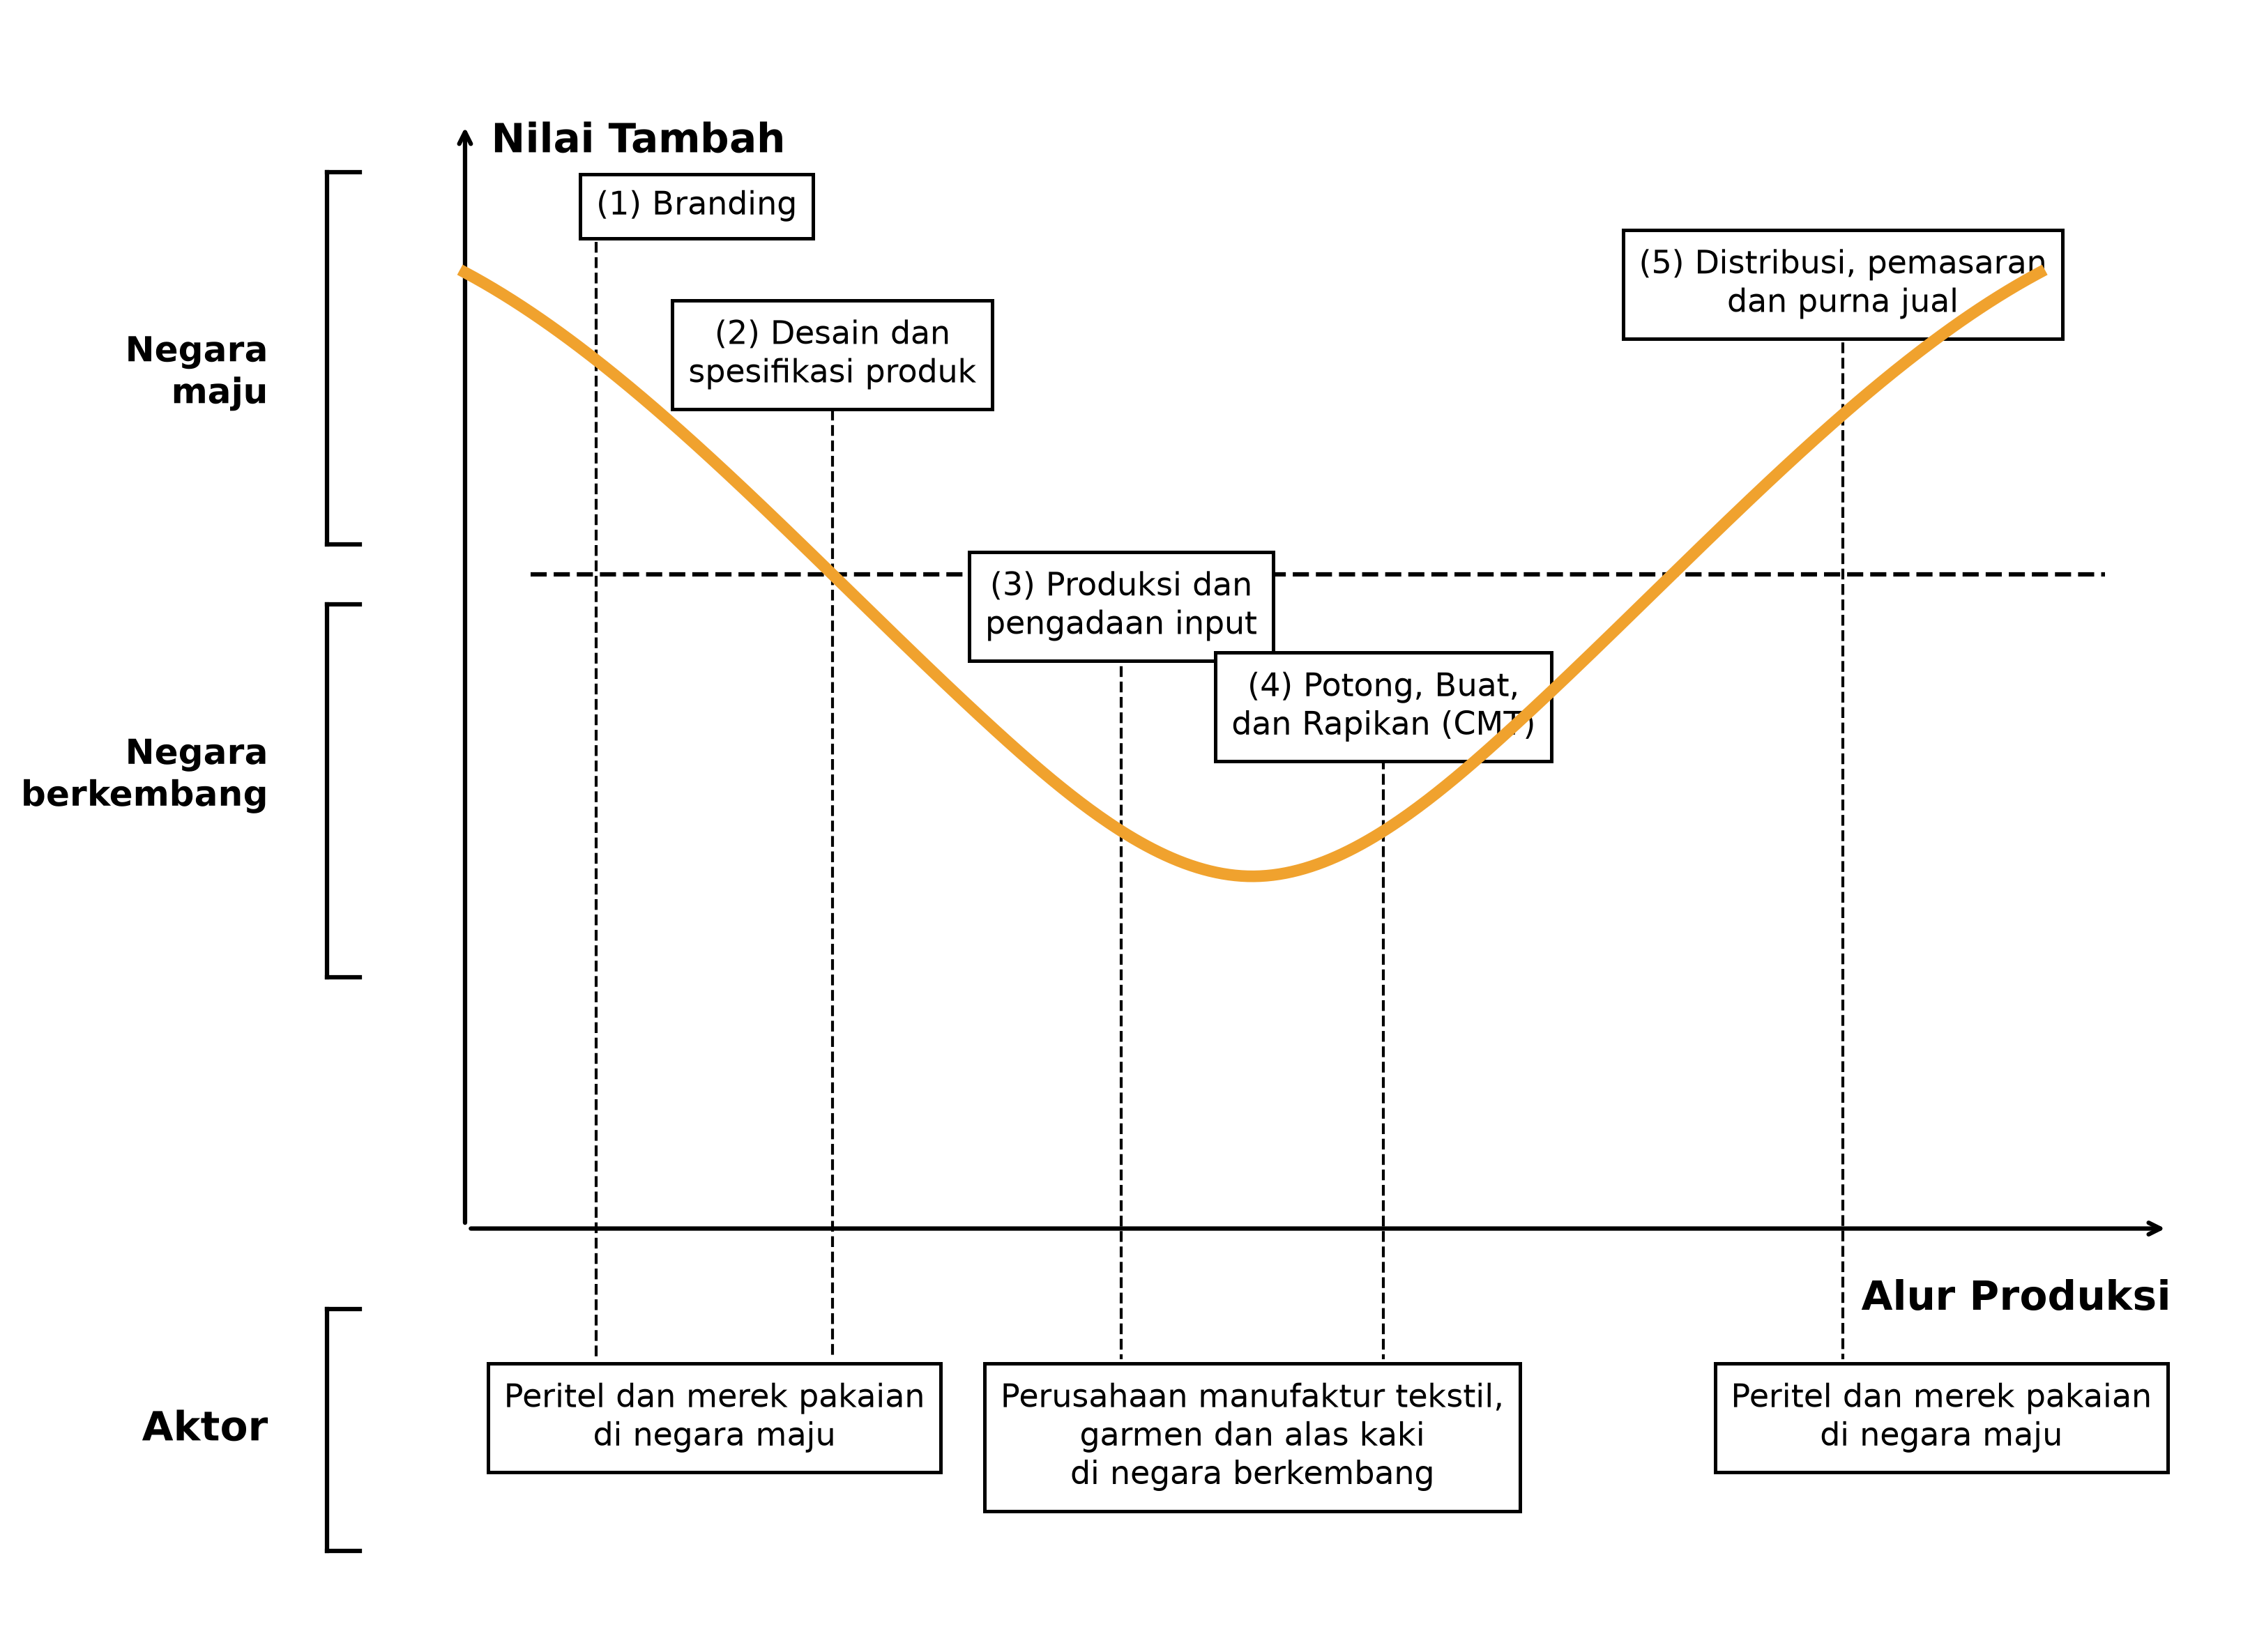
\includegraphics[width=0.9\linewidth,height=\textheight,keepaspectratio]{fig/smile_curve_indonesia.png}

}

\caption{\label{fig-smile}Ilustrasi kurva senyum pada industri tekstil
dan alas kaki. Sumber: Goto (2023), perhitungan penulis.}

\end{figure}%

Kemajuan pada perdagangan, komunikasi dan logistik telah memungkinkan
tahapan produksi yang berbeda terfragmentasi secara geografis lintas
negara. Kegiatan bernilai tambah lebih tinggi cenderung terkonsentrasi
di negara dengan kapabilitas yang lebih kuat pada desain,
\emph{branding}, teknologi dan jasa terspesialisasi, sementara kegiatan
manufaktur padat karya kerap dilakukan di negara dengan pasokan tenaga
kerja produksi umum yang lebih besar. Karena proses produksi sering
melintasi batas negara berkali-kali sebelum produk sampai ke konsumen
akhir, fenomena ini umum disebut sebagai Rantai Nilai Global
(\emph{Global Value Chain}/GVC) (Feenstra dan Taylor 2021; Gereffi dan
Frederick 2010; Gupta, Choirinnida, dan Taufik 2022).

Banyak perusahaan tekstil dan alas kaki yang beroperasi di Indonesia
terintegrasi ke dalam GVC tersebut. Perusahaan-perusahaan ini umumnya
berfungsi sebagai manufaktur kontrak bagi merek global seperti Nike,
Adidas, H\&M dan Uniqlo (yang sering disebut sebagai \emph{buyer} atau
prinsipal). Prinsipal pada akhirnya memegang kendali atas desain produk,
standar kualitas, keputusan pengadaan, logistik dan pemasaran, sementara
pihak manufaktur terutama menyediakan jasa produksi. Penting dicatat
bahwa baik bahan baku maupun barang jadi pada umumnya tetap menjadi
milik prinsipal sepanjang proses produksi. Karena itu, statistik ekspor
Indonesia hanya akan menangkap ongkos manufaktur, bukan nilai yang lebih
tinggi yang melekat dan berasal, misalnya, dari desain dan
\emph{branding}.

Pada akhirnya, Indonesia terutama berpartisipasi pada segmen manufaktur
dari rantai nilai, di mana nilai tambahnya relatif rendah, sementara
kegiatan bernilai lebih tinggi seperti \emph{branding}, desain dan
pemasaran tetap terkonsentrasi pada perusahaan utama (\emph{lead firm})
global. Akibatnya, nilai ekspor (diukur atas dasar \emph{Free on Board})
terutama menangkap tahap manufaktur yang dilakukan di Indonesia. Nilai
tersebut tidak mencerminkan nilai ritel yang jauh lebih tinggi yang
dihasilkan pada tahapan hilir dari rantai nilai.

Mengingat integrasinya ke dalam rantai nilai global, Kawasan Berikat
berperan penting dalam mendukung industri tekstil dan alas kaki
Indonesia yang berorientasi ekspor. Berdasarkan Peraturan Menteri
Keuangan No.~131/2018, Kawasan Berikat merupakan kawasan yang ditetapkan
untuk menimbun barang impor dan/atau barang dari dalam negeri yang akan
diolah, sebelum diekspor atau digunakan di dalam negeri. Fasilitas yang
berlokasi di Kawasan Berikat memperoleh manfaat berupa berkurangnya
beban administratif dan perpajakan terkait impor mesin dan input
produksi, sehingga mendukung daya saing manufaktur berorientasi ekspor.
Menurut Masitoh (2024), 453 dari 1455 perusahaan penerima fasilitas
Kawasan Berikat merupakan perusahaan tekstil dan garmen, setara dengan
11,60\% dari seluruh perusahaan tekstil dan garmen di Indonesia.

Berdampingan dengan perusahaan yang terintegrasi secara global tersebut,
Indonesia juga memiliki sejumlah besar produsen domestik independen yang
tidak terintegrasi langsung ke dalam GVC. Berbeda dengan manufaktur
kontrak berorientasi ekspor, perusahaan-perusahaan ini umumnya
beroperasi dengan merek sendiri, mengadakan inputnya sendiri dan
memasarkan produknya secara langsung kepada peritel dan konsumen.
Kelompok ini sangat beragam, mulai dari manufaktur skala menengah yang
memasok jaringan ritel domestik, usaha kecil dan mikro, hingga produsen
artisanal yang berakar pada tradisi kriya daerah.

Kelompok ini pada umumnya berorientasi pada pasar domestik dan terutama
bertumpu pada investasi domestik. Selain itu, banyak di antara produsen
tersebut memiliki akses terbatas terhadap kapabilitas desain milik
sendiri atau teknologi produksi mutakhir, serta bergantung pada input
dan mesin impor yang mungkin tidak tercakup oleh fasilitasi yang
tersedia bagi pelaku Kawasan Berikat. Proses produksi mereka cenderung
kurang kompleks dan tunduk pada persyaratan kepatuhan yang lebih sedikit
terkait standar kualitas yang ditetapkan pembeli global ataupun ESPR.

Hal ini memunculkan suatu bentuk dualisme ekonomi di dalam industri
tekstil dan alas kaki Indonesia. Di satu sisi, terdapat perusahaan
berskala besar, yang kerap merupakan penanaman modal asing, yang
terintegrasi ke dalam GVC dan terhubung dengan pembeli internasional. Di
sisi lain terdapat perusahaan yang lebih kecil dan artisan yang terutama
melayani pasar domestik. Kedua kelompok ini berbeda secara signifikan
dari sisi model bisnis, struktur produksi dan tantangan persaingan.
Akibatnya, intervensi kebijakan yang efektif bagi eksportir yang
terintegrasi secara global boleh jadi tidak menjawab dan/atau menangkap
kendala yang dihadapi produsen berorientasi domestik, dan sebaliknya.
Mengenali perbedaan ini karena itu menjadi esensial bagi perumusan
kebijakan yang efektif. Sementara itu, memahami akar struktural yang
lebih dalam menuntut penelaahan atas bagaimana Indonesia diposisikan di
dalam rantai global.

\subsection{Gambaran Umum Industri Tekstil \&
Garmen}\label{gambaran-umum-industri-tekstil-garmen}

Industri tekstil Indonesia membentang di sepanjang kurva senyum, dan
terdiri atas rantai produksi yang terintegrasi secara vertikal mulai
dari pengolahan bahan baku di hulu hingga manufaktur garmen dan kegiatan
ritel di hilir (Gambar~\ref{fig-textilechain}). Segmen hulu, termasuk
pengolahan input petrokimia seperti PTA/MEG, produksi serat poliester
dan pemintalan benang, cenderung padat modal dan padat energi. Sementara
itu, produksi menjadi semakin padat karya ke arah hilir, yang berpuncak
pada manufaktur garmen dan sektor ritel. Perbedaan struktural ini
berimplikasi langsung pada jenis nilai tambah yang dihasilkan, profil
ketenagakerjaan yang ditopang, dan sifat tekanan persaingan yang
dihadapi pada setiap tahap.

\begin{figure}[htbp!]

\centering{

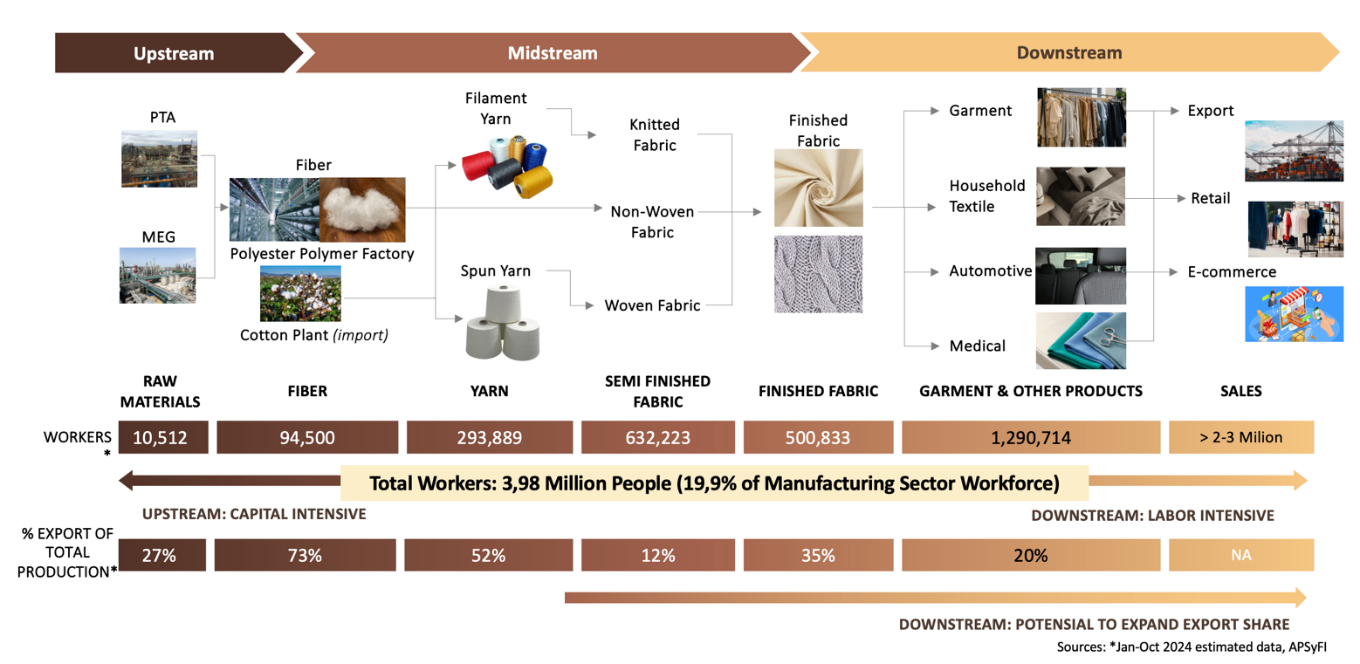
\includegraphics[width=1\linewidth,height=\textheight,keepaspectratio]{fig/textile_value_chain.png}

}

\caption{\label{fig-textilechain}Struktur rantai nilai industri tekstil.
Sumber: BPS, International Textile Manufacturers Federation.}

\end{figure}%

Segmen hulu tekstil Indonesia menunjukkan orientasi ekspor yang relatif
kuat. Pangsa ekspor produksi serat dan benang masing-masing mencapai
73\% dan 52\% (Gambar~\ref{fig-textilechain}). Sebaliknya, kegiatan
hilir seperti manufaktur garmen mengekspor 20,00\% dari total
produksinya. Namun, penyerapan tenaga kerja meningkat di sepanjang
rantai nilai, naik dari sekitar 10.000 pekerja pada pengolahan bahan
baku (PTA/MEG) menjadi lebih dari 1,29 juta pekerja pada manufaktur
garmen.

Peran yang saling melengkapi di antara berbagai segmen rantai nilai
menegaskan arti penting strategis industri tekstil secara lebih luas.
Segmen hulu berkontribusi pada penerimaan ekspor dan integrasi ke dalam
GVC, sementara segmen hilir menjadi sumber utama lapangan kerja formal
dan pendapatan. Perbedaan-perbedaan ini menegaskan perlunya pendekatan
kebijakan yang terdiferensiasi, yang mengenali perbedaan kendala,
kapabilitas dan peluang yang dihadapi perusahaan di berbagai segmen
rantai nilai.

Distribusi geografis industri tekstil Indonesia menunjukkan bahwa
kegiatan produksi masih sangat terkonsentrasi di Pulau Jawa
(Gambar~\ref{fig-maptextile}). Dari 761 perusahaan tekstil yang
tercatat, hampir 57\% berlokasi di Jawa Barat, yang berfungsi sebagai
pusat utama industri tekstil Indonesia, ditopang oleh ketersediaan
tenaga kerja, infrastruktur pendukung, serta kedekatan dengan pasar dan
rantai pasok. Jawa Tengah (18\%) dan Banten (10\%) juga berperan penting
sebagai klaster industri utama, sementara Jawa Timur (9,2\%) terus
berkontribusi melalui konsentrasi industri skala menengahnya. Secara
bersama-sama, provinsi-provinsi tersebut membentuk inti basis manufaktur
tekstil Indonesia.

\begin{figure}[htbp!]

\centering{

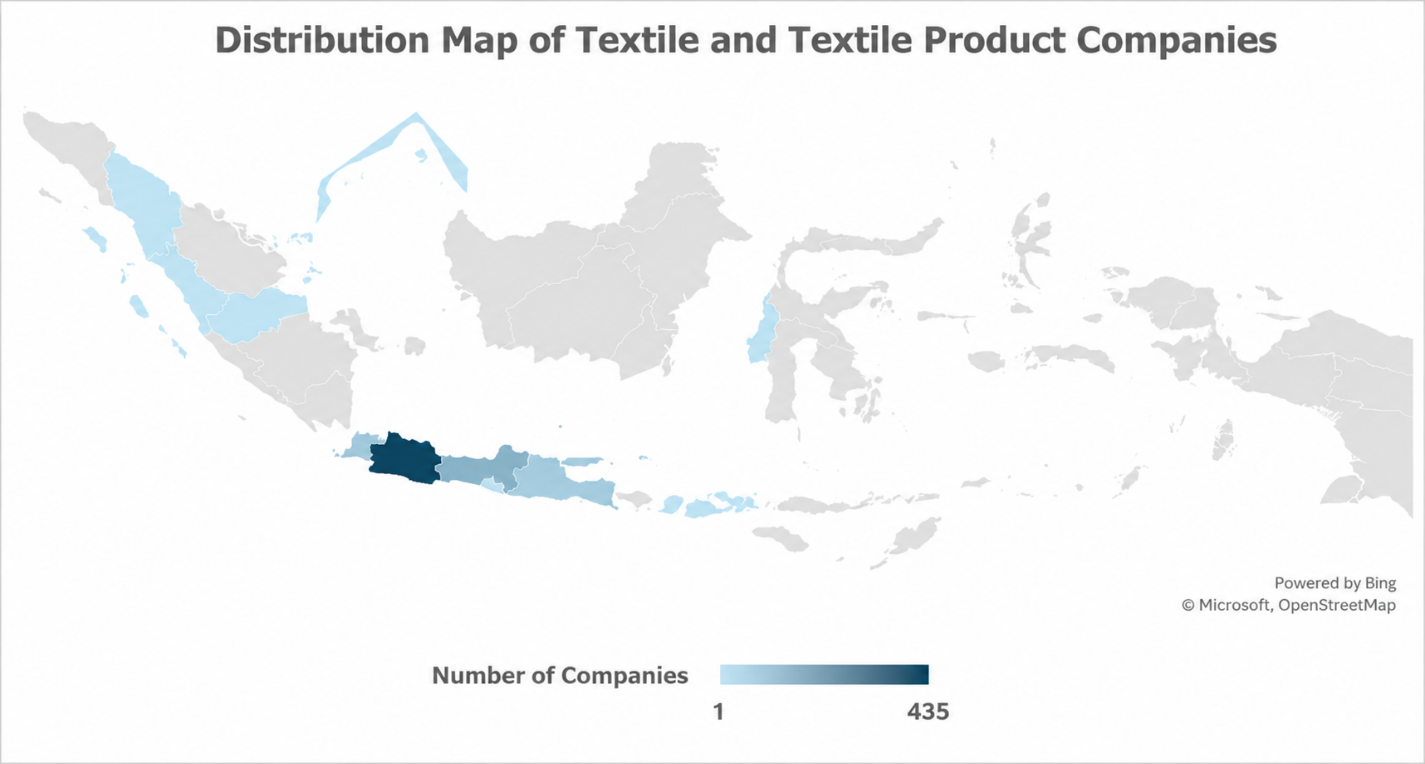
\includegraphics[width=1\linewidth,height=\textheight,keepaspectratio]{fig/map_textile.png}

}

\caption{\label{fig-maptextile}Peta sebaran perusahaan pada industri
tekstil. Sumber: BPS, perhitungan penulis.}

\end{figure}%

Di luar Jawa (2,37\%), jumlah manufaktur tekstil jauh lebih sedikit dan
tersebar secara geografis. Banyak di antara usaha tersebut tumbuh dari
tradisi lokal seperti tenun dan kerajinan tekstil. Hal ini menggambarkan
heterogenitas struktural pada tingkat perusahaan, di mana manufaktur
berskala besar yang terintegrasi ke dalam GVC hidup berdampingan dengan
produsen berorientasi domestik, UMKM dan usaha artisanal, yang
masing-masing menghadapi kondisi persaingan dan kebutuhan kebijakan yang
berbeda.

\subsection{Gambaran Umum Industri Alas
Kaki}\label{gambaran-umum-industri-alas-kaki}

Industri alas kaki Indonesia serupa dicirikan oleh proses produksi
bertahap yang mencakup pemasok bahan baku, manufaktur komponen,
perakitan alas kaki dan distribusi kepada konsumen akhir
(Gambar~\ref{fig-footwearchain}; Gambar~\ref{fig-footwearprocess}).
Input seperti kulit, karet, tekstil, bahan sintetis dan komponen kimia
diolah menjadi bagian-bagian alas kaki sebelum dirakit menjadi produk
jadi. Meskipun penciptaan nilai pada industri ini melampaui kegiatan
manufaktur hingga ke kegiatan seperti desain, pengembangan produk,
\emph{branding}, dan inovasi, kegiatan produksi tetap menjadi segmen
dominan yang dilakukan di Indonesia.

\begin{figure}[htbp!]

\centering{

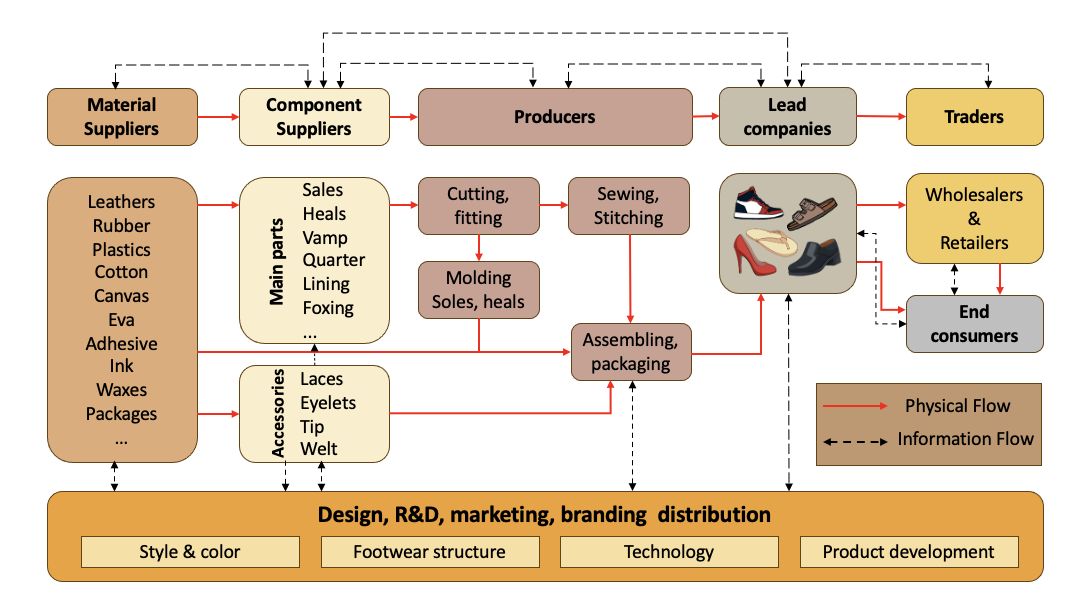
\includegraphics[width=1\linewidth,height=\textheight,keepaspectratio]{fig/footwear_supply_chain.png}

}

\caption{\label{fig-footwearchain}Rantai pasok alas kaki. Sumber:
Gereffi (1994); Stacey (2019).}

\end{figure}%

\begin{figure}[htbp!]

\centering{

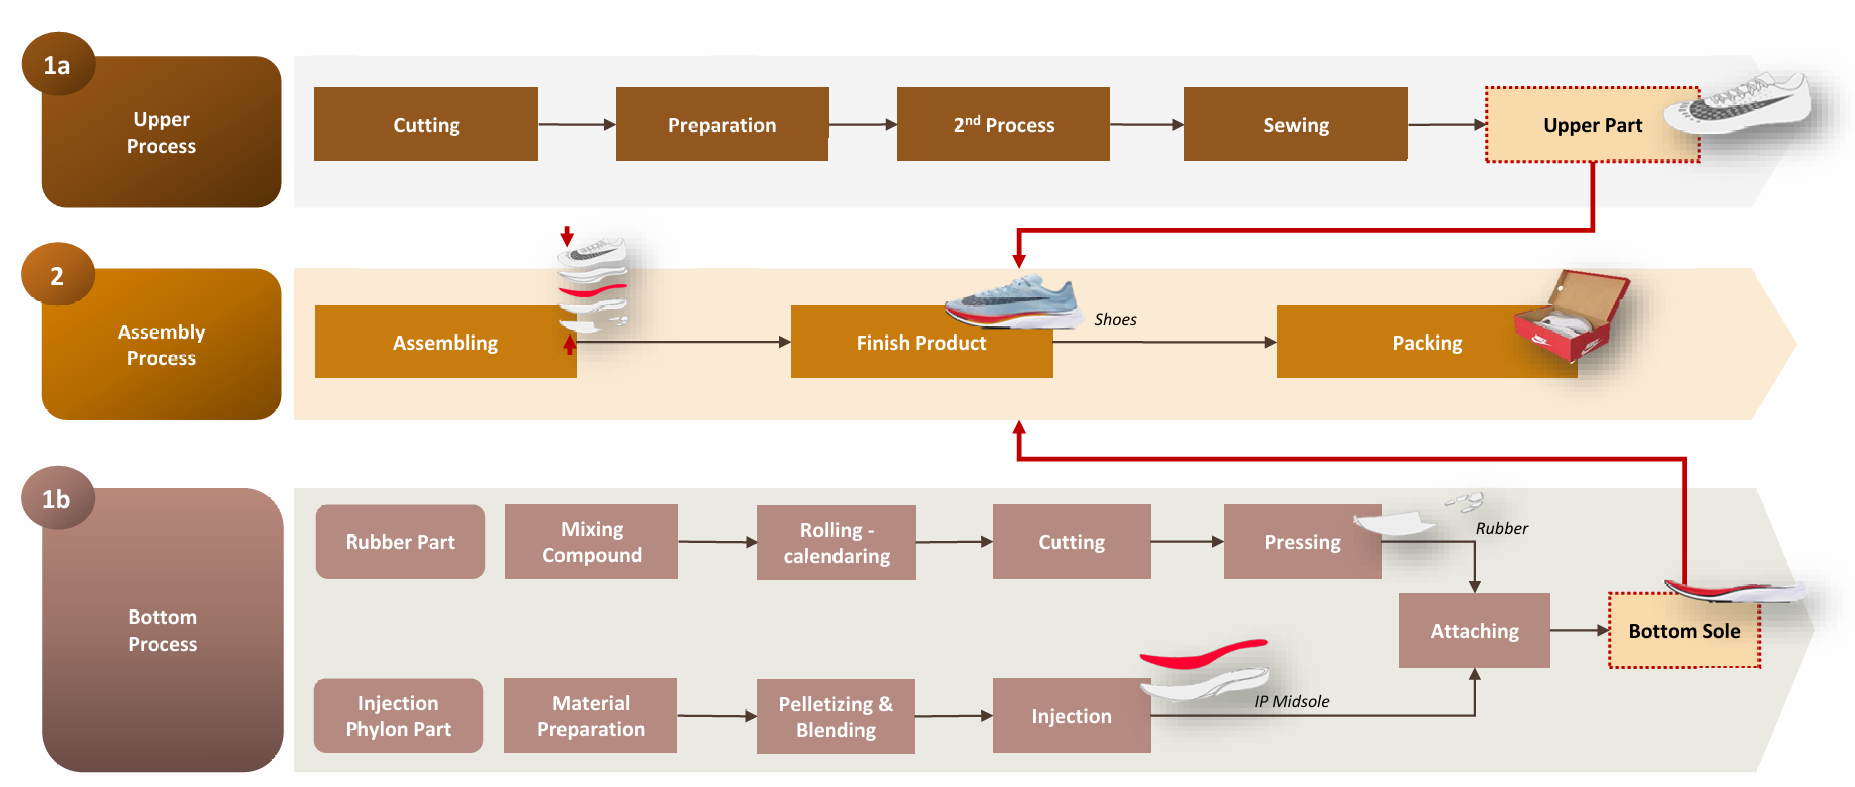
\includegraphics[width=1\linewidth,height=\textheight,keepaspectratio]{fig/footwear_production_process.png}

}

\caption{\label{fig-footwearprocess}Proses produksi pabrik pada industri
alas kaki. Sumber: DEN (2025), berdasarkan kunjungan lapangan dan
wawancara dengan manufaktur alas kaki.}

\end{figure}%

Banyak manufaktur alas kaki Indonesia yang terintegrasi ke dalam GVC,
memasok merek internasional melalui jaringan produksi berorientasi
ekspor. Sebagaimana disebutkan sebelumnya, perusahaan-perusahaan ini
umumnya berspesialisasi pada kegiatan manufaktur di dalam rantai nilai,
sementara fungsi bernilai tambah lebih tinggi kerap dilakukan oleh
perusahaan utama global. Ketergantungan industri alas kaki yang besar
pada PMA (mencakup sekitar 90\% total investasi) mencerminkan integrasi
yang dalam ke dalam jaringan produksi internasional tersebut.

Pada saat yang sama, industri alas kaki Indonesia terus menghadapi
tantangan struktural pada segmen hulu. Ketergantungan pada input impor
masih tinggi, diperkirakan berkisar antara 60--70\% (Ministry of
Industry 2024). Konsisten dengan kerangka kurva senyum, kekuatan
komparatif Indonesia tetap terkonsentrasi pada kegiatan produksi hilir,
sementara kapabilitas hulu masih relatif kurang berkembang. Hal ini
merupakan pertimbangan struktural bagi daya saing jangka panjang yang
perlu terus mendapat perhatian, sekalipun produk alas kaki Indonesia
terus berkinerja baik di pasar internasional.

Basis produksi industri alas kaki sangat terkonsentrasi di Pulau Jawa
(Gambar~\ref{fig-mapfootwear}). Jawa Barat menjadi lokasi bagi jumlah
pabrik alas kaki terintegrasi global terbanyak, dengan 42 fasilitas yang
mempekerjakan lebih dari 186.000 pekerja di Sukabumi, Garut, Cibogo dan
Karawang. Banten dan Jawa Tengah masing-masing menjadi lokasi bagi 29
dan 13 pabrik, dengan setiap provinsi mempekerjakan sedikit di atas
112.000 pekerja. Konsentrasi produksi di provinsi-provinsi tersebut
ditopang oleh infrastruktur industri, akses terhadap pemasok dan
jaringan ekspor yang telah mapan.

\begin{figure}[htbp!]

\centering{

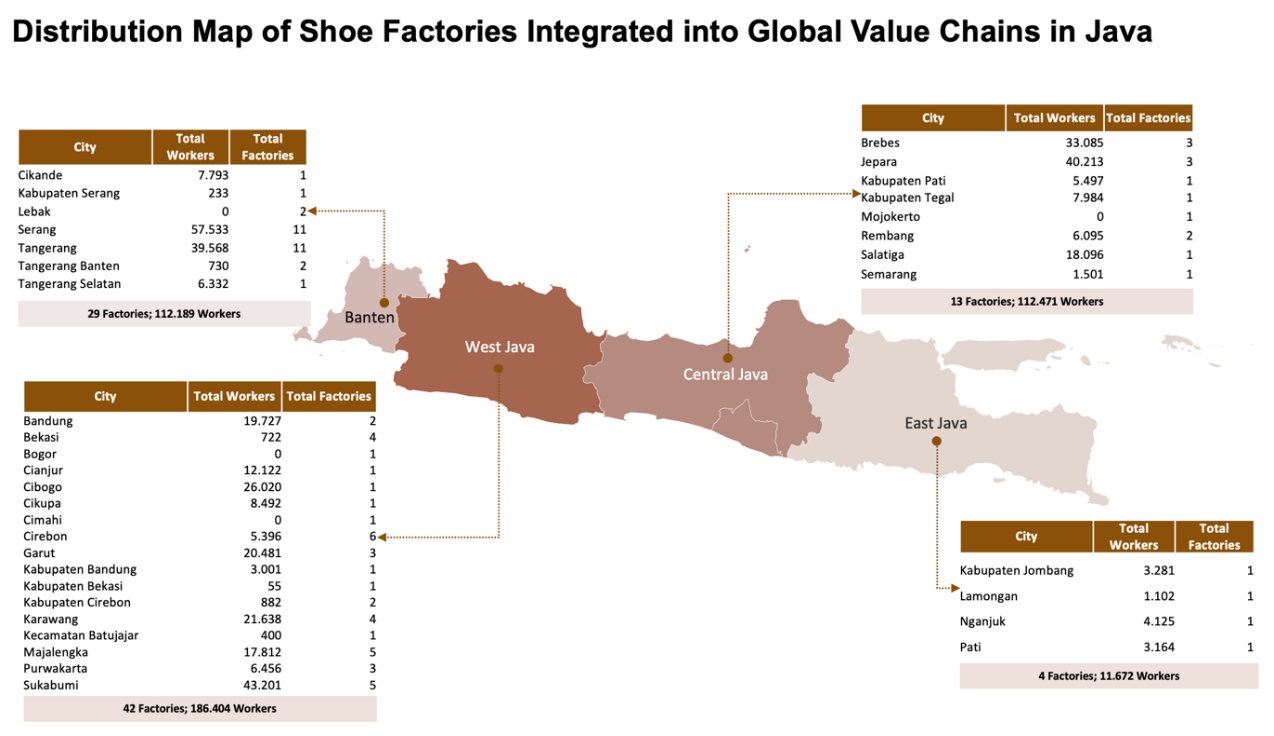
\includegraphics[width=1\linewidth,height=\textheight,keepaspectratio]{fig/map_footwear.png}

}

\caption{\label{fig-mapfootwear}Sebaran geografis pabrik alas kaki di
Jawa. Sumber: APRISINDO (2025); analisis DEN.}

\end{figure}%

Tren investasi terkini menunjukkan bahwa Jawa Tengah muncul sebagai
tujuan yang semakin penting bagi ekspansi manufaktur alas kaki. Meskipun
Jawa Barat dan Banten tetap menjadi pusat produksi terbesar industri
ini, biaya tenaga kerja yang relatif lebih rendah dan ketersediaan
pekerja telah mendorong perusahaan mendirikan fasilitas baru dan
memperluas operasi yang ada di Jawa Tengah. Penyerapan tenaga kerja pada
industri alas kaki di Jawa Tengah diperkirakan meningkat sekitar 85.000
pekerja\footnote{Berdasarkan wawancara DEN dan estimasi penulis dengan
  menggunakan rencana ekspansi dua manufaktur alas kaki global besar dan
  jaringan pemasoknya di Jawa Tengah (2025).} dalam satu hingga dua
tahun ke depan, yang menegaskan semakin pentingnya wilayah tersebut
dalam lanskap manufaktur alas kaki Indonesia.

Hal ini menegaskan sejauh mana perkembangan di Jawa terus membentuk
kinerja industri alas kaki Indonesia. Mengingat konsentrasi manufaktur
di pulau tersebut, upaya memperkuat daya saing (misalnya melalui
perbaikan infrastruktur, pengembangan sumber daya manusia dan insentif
investasi) akan sangat bergantung pada koordinasi yang efektif antara
pemerintah pusat dan pemerintah provinsi di pusat-pusat produksi utama
tersebut.

\section{Isu Strategis pada Industri Tekstil \& Garmen dan Alas
Kaki}\label{isu-strategis-pada-industri-tekstil-garmen-dan-alas-kaki}

Tantangan strategis yang dihadapi industri tekstil dan alas kaki
Indonesia dibentuk oleh dualisme ekonomi dan struktur industri yang
heterogen pada sektor ini. Dua implikasinya sangat penting. Pertama,
keberadaan rantai nilai yang relatif lengkap tidak serta-merta berarti
adanya integrasi yang kuat di seluruh segmen. Kedua, segmen industri
yang berbeda kerap menghadapi kendala dan kebutuhan kebijakan yang
secara mendasar berbeda.

Gambar~\ref{fig-trade} mengilustrasikan implikasi pertama. Meskipun
Indonesia telah mengembangkan industri tekstil hulu yang substansial,
negara ini terus secara bersamaan mengimpor dan mengekspor bahan baku
dan barang antara tekstil dalam volume yang signifikan. Industri rayon
memberikan contoh yang berguna. Indonesia merupakan produsen produk
berbasis viscose yang kompetitif, namun perusahaan pada segmen ini tetap
terintegrasi secara dalam ke pasar internasional. Asia Pacific Rayon
(APR), misalnya, mengekspor 61\% produksi \emph{Viscose Staple Fibre}
(VSF) dan 71\% output \emph{Viscose Yarn}-nya, sementara Indonesia terus
mengimpor produk rayon dan benang dari luar negeri (Asia Pacific Rayon
2024).

\begin{figure}[htbp!]

\centering{

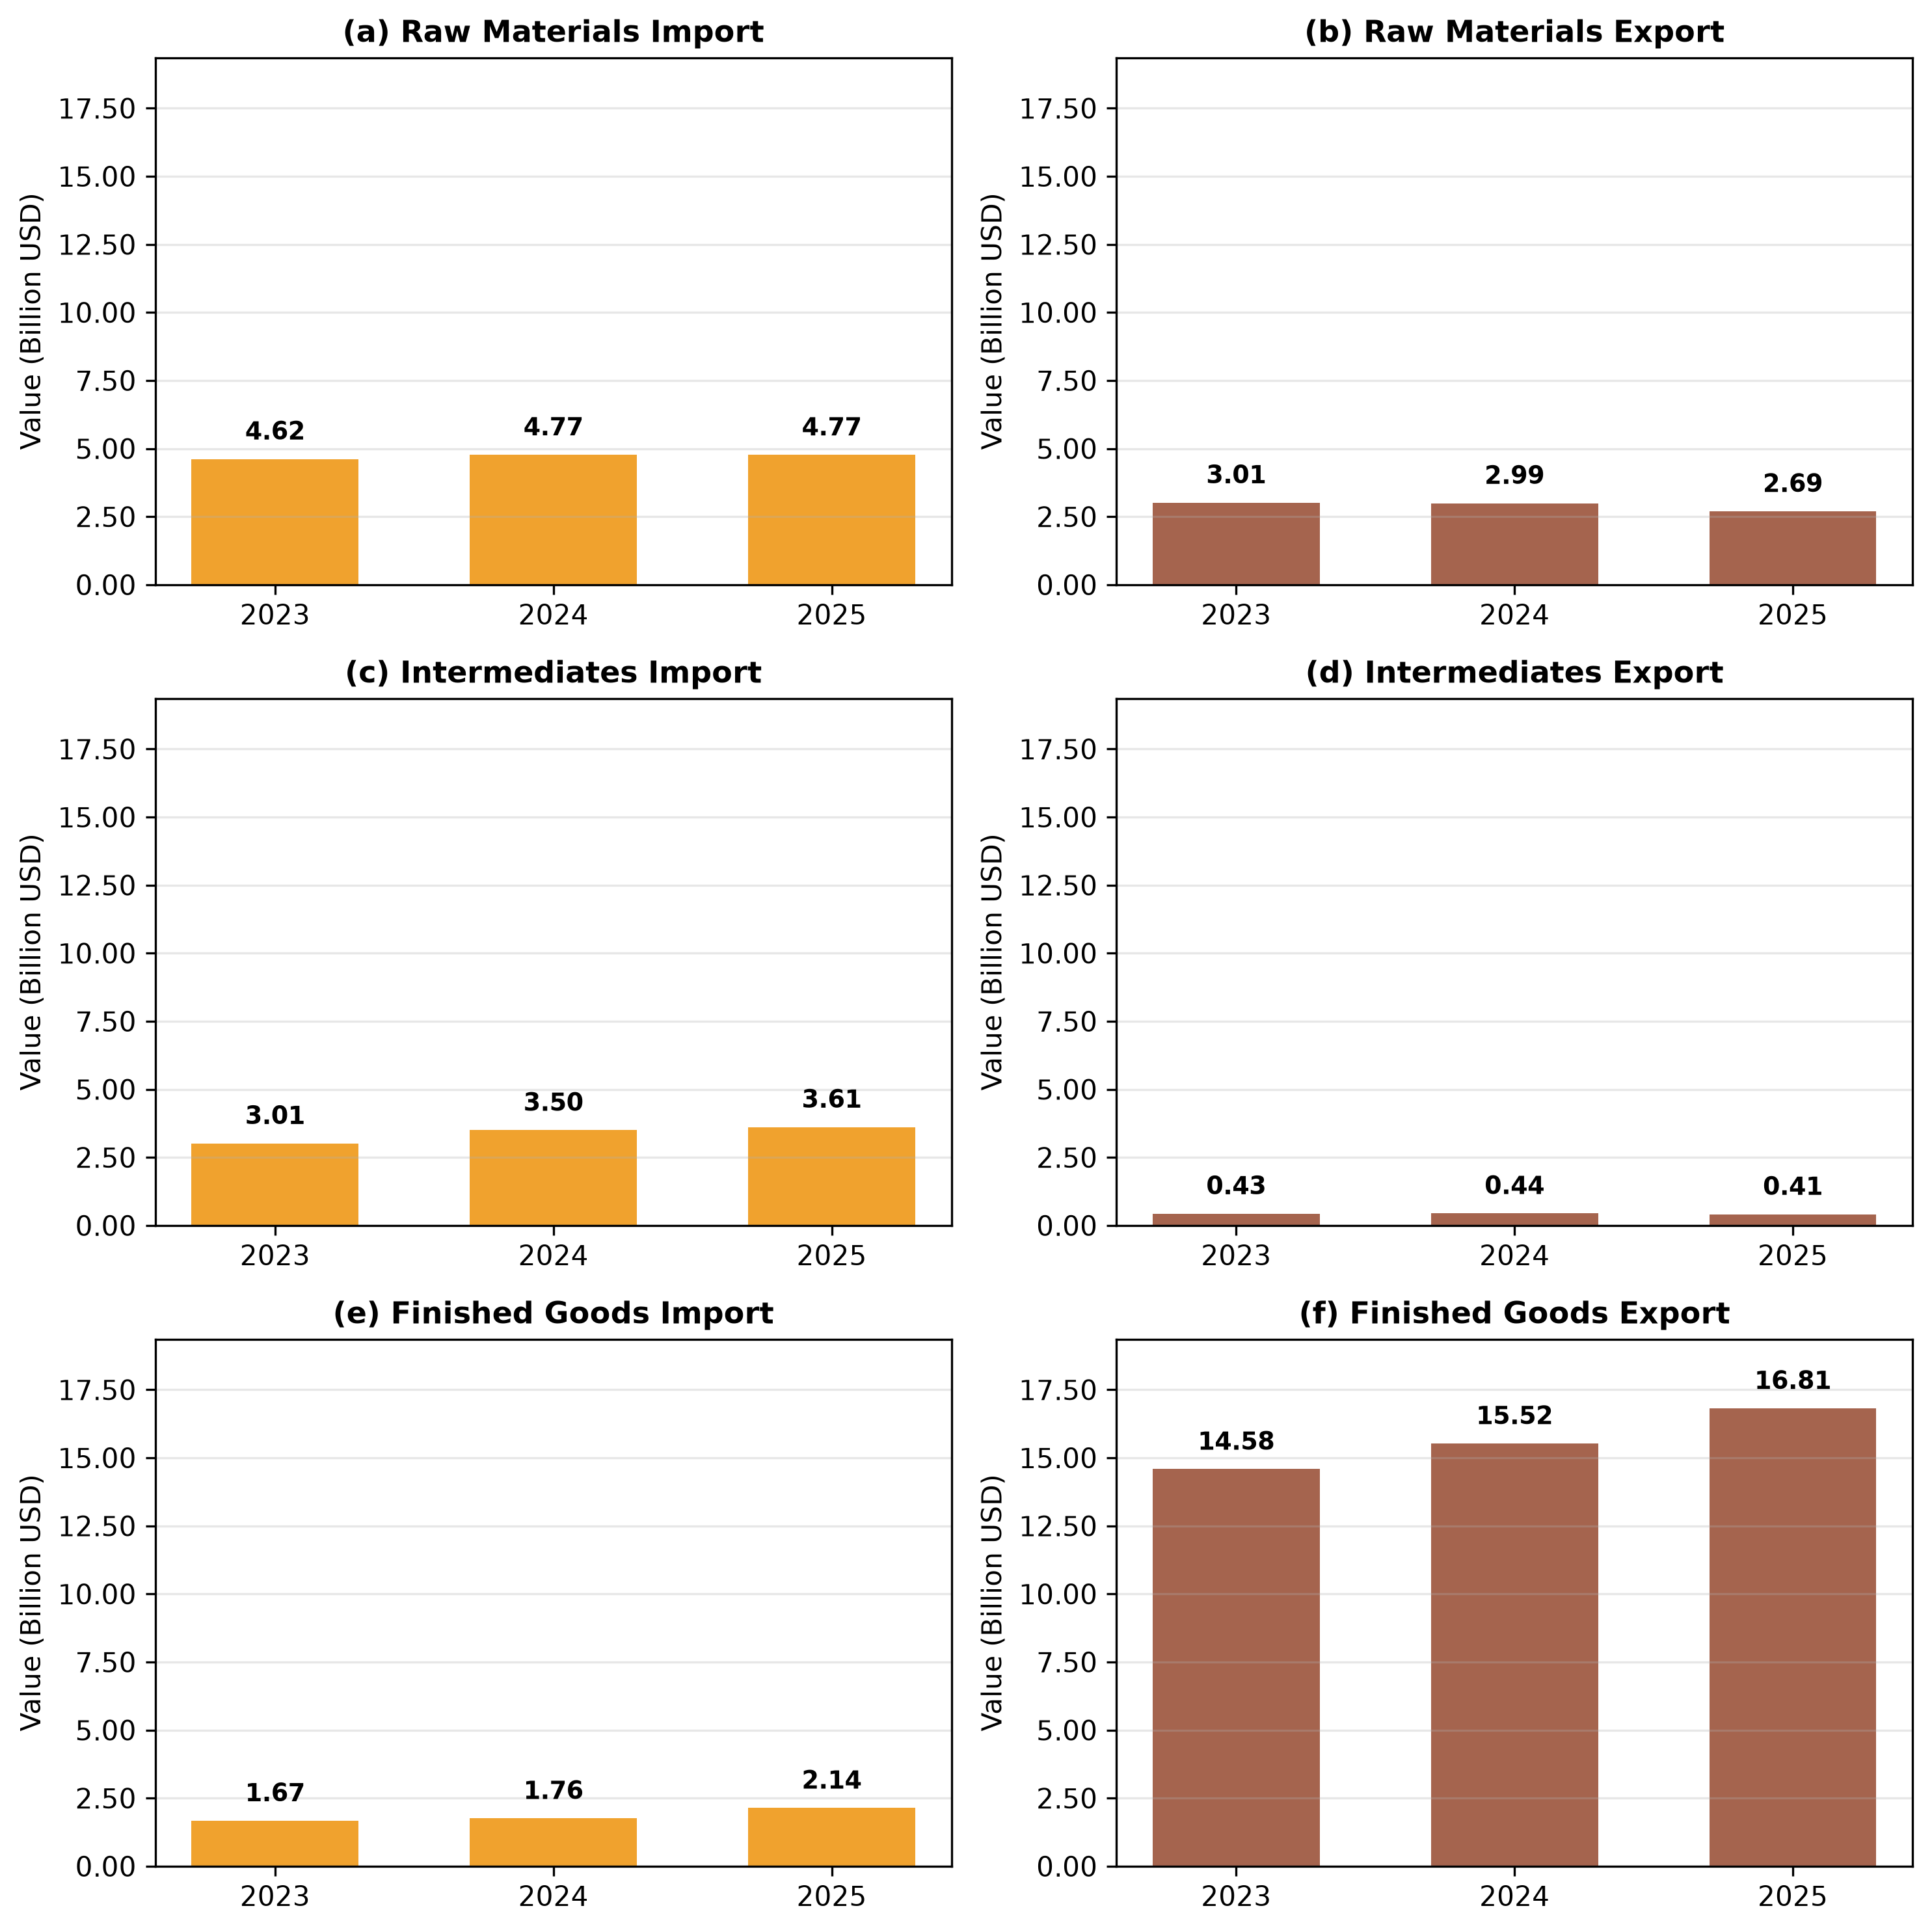
\includegraphics[width=0.75\linewidth,height=\textheight,keepaspectratio]{fig/trade_by_type.png}

}

\caption[\label{fig-trade}Ekspor dan impor barang terkait tekstil dan
alas kaki. Setiap panel menunjukkan nilai perdagangan
Indonesia dalam miliar USD menurut tahun, dipilah menurut tahapan produk
(bahan baku, barang antara, barang jadi) dan arus (impor, ekspor).
Sumber: UN COMTRADE.]{\label{fig-trade}Ekspor dan impor barang terkait tekstil dan
alas kaki\footnotemark{}. Setiap panel menunjukkan nilai perdagangan
Indonesia dalam miliar USD menurut tahun, dipilah menurut tahapan produk
(bahan baku, barang antara, barang jadi) dan arus (impor, ekspor).
Sumber: UN COMTRADE.}

\end{figure}%
\footnotetext{Bahan baku didefinisikan sebagai Bab Kode HS 50--55;
  barang antara mencakup bab 56, 58, 59, dan 60; dan barang jadi
  meliputi bab 61--64.}

Salah satu penjelasan atas pola tersebut adalah bahwa segmen industri
yang berbeda kerap berpartisipasi pada rantai nilai yang berbeda.
Produsen bahan baku domestik boleh jadi telah terintegrasi ke dalam
jaringan produksi internasional dan memasok pembeli di luar negeri,
sementara manufaktur benang dan kain domestik boleh jadi memperoleh
input dari pemasok yang ditunjuk oleh klien atau prinsipal mereknya di
luar negeri. Hubungan-hubungan tersebut kerap sangat terspesialisasi dan
tidak mudah disubstitusi. Akibatnya, statistik perdagangan saja tidak
dapat sepenuhnya menangkap derajat integrasi di dalam industri, dan
kebijakan yang semata-mata didasarkan pada klasifikasi kode HS berisiko
mengganggu rantai nilai yang telah terbangun.\footnote{Hal ini juga
  menjadi persoalan pada industri lain yang bertumpu pada rantai nilai
  global, seperti industri makanan dan minuman, permesinan, dan
  elektronik (Gupta, Pane, dan Pasaribu 2022; Hasran, Gupta, dan Aaron
  2025).}

Implikasi kedua dari dualisme ekonomi ini adalah bahwa segmen industri
yang berbeda kerap memerlukan respons kebijakan yang berbeda. Perusahaan
yang terintegrasi ke dalam rantai nilai global umumnya beroperasi dengan
serangkaian peluang dan kendala yang berbeda dibandingkan produsen
berorientasi domestik. Perusahaan utama dan merek global memainkan peran
koordinasi yang penting dengan menyediakan akses pasar, menetapkan
standar produksi, memfasilitasi alih pengetahuan, dan mengurangi risiko
komersial yang dihadapi pemasok (Gereffi, Humphrey, dan Sturgeon 2005;
Fernandez-Stark, Frederick, dan Gereffi 2011). Banyak manufaktur
berorientasi ekspor juga memperoleh manfaat dari akses yang lebih kuat
terhadap pasar internasional, pembiayaan, dan jaringan produksi.

Sebaliknya, perusahaan tekstil dan alas kaki berorientasi domestik yang
beroperasi dengan merek sendiri cenderung menghadapi tantangan yang
lebih besar terkait pembiayaan, peningkatan teknologi, perbaikan
produktivitas, dan perluasan pasar. Akses yang terbatas terhadap modal
dapat membatasi investasi pada mesin dan proses produksi baru, sementara
skala yang lebih kecil kerap mempersulit pemenuhan persyaratan yang
dibutuhkan untuk berpartisipasi dalam rantai nilai global. Persaingan
dari impor, terutama impor ilegal, juga tetap menjadi kekhawatiran yang
signifikan bagi perusahaan-perusahaan tersebut.

Perbedaan juga tampak di sepanjang rantai produksi itu sendiri. Kegiatan
hulu seperti produksi serat sangat padat modal dan padat energi,
sehingga membutuhkan investasi yang besar dan permintaan hilir yang
memadai agar tetap layak secara komersial. Akibatnya, jumlah perusahaan
yang beroperasi pada segmen tersebut cenderung relatif terbatas.
Manufaktur hilir, terutama operasi \emph{cut-make-trim} (CMT), pada
umumnya lebih terfragmentasi dan kurang padat modal, sehingga
memungkinkan perusahaan menambah kapasitas secara bertahap seiring
pertumbuhan permintaan. Oleh karena itu, sementara daya saing hulu kerap
dibentuk oleh akses terhadap modal, energi, dan bahan baku, daya saing
hilir lebih banyak bergantung pada ketersediaan tenaga kerja,
keterampilan pekerja, dan produktivitas.

Perbedaan-perbedaan tersebut menegaskan pentingnya menghindari
pendekatan seragam (\emph{one-size-fits-all}) dalam menangani isu
strategis pada industri tekstil dan alas kaki.

\subsection{Perdagangan Internasional}\label{perdagangan-internasional}

Mengingat karakter ekonomi yang dualistik dan struktur industri yang
sangat terkait dengan rantai nilai global, perdagangan internasional
membawa implikasi yang signifikan bagi industri ini. Sebagaimana dibahas
sebelumnya, AS dan UE tetap menjadi pasar ekspor terpenting industri
ini. Akibatnya, perkembangan kebijakan perdagangan dan akses pasar pada
kedua perekonomian tersebut memiliki implikasi yang signifikan bagi
investasi dan produksi industri ini di Indonesia.

Untuk pasar AS, tantangan utama berpusat pada ketidakpastian kebijakan
terkait tarif dan daya saing biaya. Industri Indonesia rentan terhadap
ancaman tarif resiprokal dan potensi hilangnya manfaat \emph{Generalized
System of Preferences} (GSP), yang akan secara langsung menaikkan bea
masuk dan menekan margin. Pada saat yang sama, Indonesia menghadapi
persaingan ketat dari negara seperti Vietnam, yang sangat kompetitif
dari sisi biaya produksi domestik. Tekanan gabungan dari beban tarif dan
inefisiensi biaya berpotensi signifikan menantang ekspor dan investasi,
yang menegaskan perlunya transformasi struktural untuk meningkatkan daya
saing global.

Untuk pasar UE, prospeknya lebih menguntungkan. Penyelesaian secara
substansi \emph{Indonesia--European Union Comprehensive Economic
Partnership Agreement} (IEU-CEPA) diharapkan memberikan akses bebas bea
bagi ekspor tekstil dan alas kaki Indonesia. Hal ini sangat penting
karena akan menempatkan eksportir Indonesia pada posisi yang lebih
setara dengan pesaing seperti Vietnam, yang telah memperoleh manfaat
dari akses tarif preferensial ke pasar UE.

Namun, akses terhadap preferensi tersebut bergantung pada kepatuhan
terhadap Ketentuan Asal Barang (\emph{Rules of Origin}/RoO), khususnya
persyaratan ``transformasi ganda'' (\emph{double transformation}).
Berdasarkan ketentuan ini, produk harus melalui sekurang-kurangnya dua
tahap produksi di dalam negeri untuk memenuhi syarat tarif preferensial.
Untuk garmen, misalnya, kainnya pun harus diproduksi di dalam negeri,
bukan diimpor. Tujuannya adalah mencegah \emph{transshipment} dan
memastikan bahwa preferensi tarif terkait dengan penciptaan nilai tambah
domestik yang sesungguhnya.

Bagi perusahaan yang beroperasi dengan skema CMT (\emph{cut-make-trim}),
persyaratan ini merupakan tantangan yang signifikan. Banyak manufaktur
masih bertumpu pada kain dan input antara impor yang dipasok melalui
jaringan pembeli global. Kepatuhan terhadap ketentuan transformasi ganda
karena itu akan menuntut penguatan produksi barang antara di dalam
negeri atau tambahan investasi hulu oleh pemasok yang ada.

Meskipun persyaratan transformasi ganda menciptakan insentif untuk
memperkuat industri hulu dan antara domestik, impor kemungkinan akan
tetap menjadi bagian penting dari struktur produksi industri ini. Hal
ini terutama berlaku untuk input terspesialisasi, bahan bermilik
(\emph{proprietary}), dan produk yang tidak tersedia di dalam negeri
dengan kualitas, spesifikasi, atau volume yang dibutuhkan. Akibatnya,
impor memainkan peran ganda di dalam industri ini. Di satu sisi, impor
dapat bersaing secara langsung dengan produsen domestik pada segmen yang
sama. Di sisi lain, impor menyediakan akses terhadap input yang menopang
produksi, ekspor, dan partisipasi dalam rantai nilai global. Kajian oleh
DEN, Gherzi dan Prospera serupa menekankan bahwa impor dapat sekaligus
mendukung dan menantang pembangunan industri.

Kekhawatiran yang lebih mendesak bukanlah impor legal itu sendiri,
melainkan impor ilegal yang sama sekali menghindari bea masuk dan
persyaratan regulasi. Pada Agustus 2025, operasi gabungan Kementerian
Perdagangan, Badan Intelijen Negara (BIN), dan Badan Intelijen Strategis
TNI (BAIS TNI) menyita 19.391 bal impor tekstil ilegal senilai Rp112,35
miliar (Deviyana 2025). Kajian industri menunjukkan bahwa praktik
semacam itu umumnya melibatkan pelaporan yang tidak sesuai
(\emph{underreporting}), \emph{underinvoicing}, dan penggunaan pintu
masuk tidak resmi. Selain mengurangi penerimaan negara, impor ilegal
merusak persaingan yang adil dan melemahkan daya saing perusahaan
domestik.

\subsection{Isu Keberlanjutan}\label{isu-keberlanjutan}

Selain isu terkait perdagangan, keberlanjutan menjadi isu yang semakin
penting bagi industri tekstil dan alas kaki. Hal ini terutama relevan
bagi perusahaan yang mengekspor ke pasar UE, di mana persyaratan
keberlanjutan secara bertahap menjadi bagian dari persyaratan akses
pasar.

Dalam kerangka \emph{European Green Deal}, Uni Eropa telah
memperkenalkan sejumlah regulasi untuk mendorong pola produksi dan
konsumsi yang lebih berkelanjutan. Salah satu yang terpenting bagi
industri tekstil dan alas kaki adalah \emph{Ecodesign for Sustainable
Products Regulation} (ESPR), yang mulai berlaku pada 2024 dan saat ini
masih menjalani konsultasi dan implementasi lebih lanjut (Yan 2025;
European Commission 2024).

ESPR mencakup persyaratan terkait durabilitas, keterbaikan
(\emph{repairability}), daur ulang, dan ketertelusuran produk. Salah
satu elemen kuncinya adalah \emph{Digital Product Passport} (DPP), yang
mensyaratkan informasi mengenai asal produk, komposisi bahan, proses
produksi, dan jejak lingkungannya dapat ditelusuri di sepanjang rantai
nilai (Costa 2025). Pemenuhan persyaratan tersebut menuntut perusahaan
memperkuat pengumpulan data, sistem ketertelusuran, dan digitalisasi di
seluruh operasinya.

Implikasinya melampaui perusahaan yang mengekspor langsung ke Uni Eropa.
Karena persyaratan ketertelusuran berlaku di sepanjang rantai nilai,
pemasok hulu juga kemungkinan terdampak. Hal ini terutama relevan pada
industri tekstil, di mana produksi serat dan kain sangat padat modal dan
dicirikan oleh skala ekonomi yang signifikan. Alih-alih mengoperasikan
sistem produksi terpisah untuk pasar yang berbeda, banyak produsen
mungkin menilai lebih praktis untuk menerapkan standar tersebut pada
seluruh operasinya.

Beberapa manufaktur berorientasi ekspor telah mulai menyesuaikan diri
dengan perubahan tersebut. Sebuah pabrik serat dan kain di Jawa
Tengah\footnote{Untuk menjaga kerahasiaan informasi yang sensitif secara
  komersial, nama perusahaan tidak diungkapkan. Informasi ini didasarkan
  pada wawancara mendalam yang dilakukan DEN dengan sebuah manufaktur
  serat dan kain berorientasi ekspor di Jawa Tengah pada 2025.} telah
mengembangkan sistem dasbor waktu nyata (\emph{real-time}) yang siap
diintegrasikan dengan sistem seperti DPP. Perusahaan tersebut juga telah
mengalihkan seluruh produksi energinya ke biomassa.

Namun, transisi menuju produksi yang lebih hijau masih menjadi tantangan
di Indonesia. Meskipun biaya energi industri relatif kompetitif, sistem
energi negara ini masih sangat bergantung pada bahan bakar fosil.
Manufaktur yang berupaya mengurangi jejak karbonnya dapat berinvestasi
pada sumber energi alternatif seperti biomassa, tenaga surya, atau gas
alam, namun masing-masing menghadapi kendalanya sendiri, termasuk
keterbatasan ketersediaan biomassa, pembatasan regulasi atas pemanfaatan
tenaga surya, serta kesenjangan pasokan dan infrastruktur gas.

Bagi banyak perusahaan, keberlanjutan tidak lagi semata-mata merupakan
isu lingkungan. Isu ini semakin menjadi persyaratan bisnis yang terkait
dengan daya saing ekspor dan partisipasi dalam rantai nilai global.

\subsection{Teknologi}\label{teknologi}

Adopsi teknologi tetap menjadi penentu penting daya saing industri
tekstil \& garmen dan alas kaki Indonesia. Selain menurunkan biaya
produksi, peningkatan teknologi semakin diperlukan untuk memperbaiki
produktivitas, kualitas produk, dan efisiensi operasional di pasar
global yang semakin kompetitif.

Gambar~\ref{fig-machinery} mengilustrasikan bahwa Indonesia secara umum
tertinggal dari pesaing di kawasan seperti Vietnam dalam hal modernisasi
permesinan, terutama pada pemintalan dan pertenunan. Selama satu dekade
terakhir, Indonesia mengalami penurunan kapasitas pada beberapa segmen
hulu, termasuk \emph{ring spinning}, \emph{open-end spinning}, dan
\emph{shuttleless loom}, sementara Vietnam terus memperluas kapasitas
melalui investasi berkelanjutan pada peralatan produksi yang lebih baru.
Tren ini menunjukkan bahwa tantangan yang dihadapi Indonesia bukan hanya
soal daya saing, tetapi juga mempertahankan kapasitas produktif pada
segmen hulu yang strategis dari rantai nilai tekstil.

\begin{figure}[htbp!]

\centering{

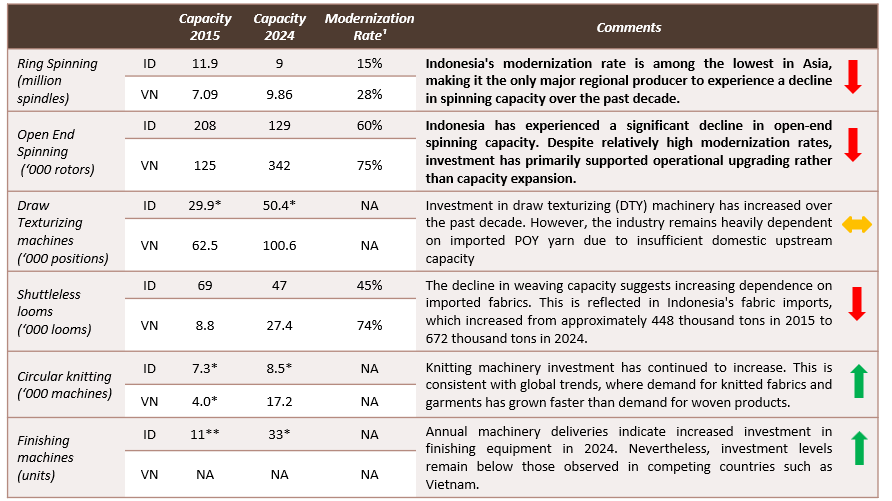
\includegraphics[width=0.9\linewidth,height=\textheight,keepaspectratio]{fig/machinery_modernization.png}

}

\caption{\label{fig-machinery}Perbandingan modernisasi permesinan
tekstil di Indonesia dan Vietnam. Sumber: DEN, ITMF, Gherzi.}

\end{figure}%

Mesin yang lebih tua cenderung kurang produktif, lebih boros energi, dan
lebih mahal untuk dipelihara, sehingga menurunkan daya saing relatif
terhadap produsen yang telah berinvestasi pada teknologi yang lebih
baru. Akibatnya, modernisasi permesinan tetap menjadi salah satu
prioritas paling mendesak bagi industri ini, terutama bagi segmen hulu
yang menjadi fondasi rantai nilai tekstil domestik.

Otomasi juga menjadi semakin penting, tidak harus sebagai pengganti
tenaga kerja, melainkan sebagai sarana untuk meningkatkan produktivitas,
konsistensi kualitas, dan efisiensi operasional. Beberapa manufaktur
besar telah mengadopsi peralatan pemotongan otomatis, sistem penanganan
material, dan teknologi manajemen gudang untuk mengurangi hambatan
produksi dan memperbaiki pengendalian proses. Wawancara yang dilakukan
DEN dengan manufaktur berorientasi ekspor menunjukkan bahwa otomasi
membantu menurunkan tingkat kecacatan, memperbaiki konsistensi produk,
dan meningkatkan efisiensi produksi, yang semuanya kritis untuk memenuhi
persyaratan kualitas pembeli global\footnote{Berdasarkan wawancara yang
  dilakukan DEN dengan manufaktur tekstil berorientasi ekspor pada 2025.
  Nama perusahaan tidak diungkapkan untuk menjaga kerahasiaan informasi
  yang sensitif secara komersial.}. Meskipun adopsinya secara lebih luas
masih timpang, terutama di kalangan perusahaan yang lebih kecil, otomasi
kemungkinan akan menjadi komponen yang semakin penting dalam peningkatan
industri pada tahun-tahun mendatang.

\subsection{Kesiapan Tenaga Kerja}\label{kesiapan-tenaga-kerja}

Industri tekstil, garmen, dan alas kaki tetap menjadi salah satu
penyerap tenaga kerja manufaktur terpenting di Indonesia. Total
penyerapan tenaga kerja meningkat dari 4,1 juta pekerja pada 2020
menjadi lebih dari 5,0 juta pada 2025, setara dengan sekitar seperempat
tenaga kerja manufaktur formal secara nasional (BPS 2025a). Manufaktur
tekstil dan garmen terus mendominasi penyerapan tenaga kerja di dalam
sektor ini, dengan hampir empat juta pekerja pada 2025. Meskipun
demikian, pertumbuhan tenaga kerja tercepat terjadi pada industri alas
kaki, di mana jumlah pekerjanya bertambah sekitar 60 persen antara 2020
dan 2025, dibandingkan pertumbuhan sekitar 15--20 persen pada manufaktur
tekstil dan garmen pada periode yang sama (Gambar~\ref{fig-workers}).

\begin{figure}[H]

\centering{

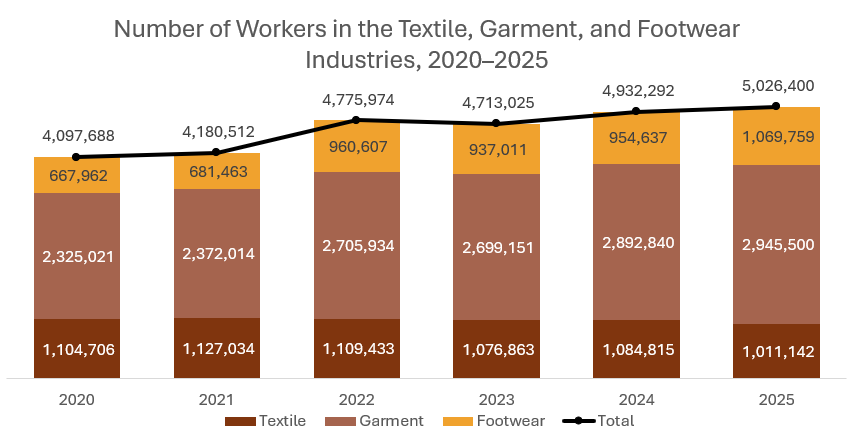
\includegraphics[width=0.7\linewidth,height=\textheight,keepaspectratio]{fig/workers.png}

}

\caption{\label{fig-workers}Jumlah pekerja pada industri padat karya
Indonesia (juta), 2020--2025. Sumber: BPS, Sakernas.}

\end{figure}%

Pertumbuhan penyerapan tenaga kerja tersebut wajar memunculkan
kekhawatiran mengenai apakah pasokan tenaga kerja dapat mengimbangi
permintaan industri. Namun, proyeksi tenaga kerja yang tersedia
menunjukkan bahwa Indonesia kecil kemungkinan akan menghadapi kekurangan
pekerja pada kedua industri tersebut. Menurut proyeksi Kementerian
Ketenagakerjaan, pasokan tahunan lulusan vokasi (lulusan SMK dan Vokasi)
yang relevan dengan industri tekstil dan alas kaki diperkirakan terus
tumbuh hingga 2029. Untuk tekstil dan garmen, pasokan lulusan
diproyeksikan meningkat dari sekitar 624.802 pada 2025 menjadi 765.763
pada 2029, setara dengan pertumbuhan rata-rata tahunan sebesar 5,2
persen. Lulusan terkait alas kaki diproyeksikan naik dari sekitar
133.232 menjadi sekitar 183 ribu pada periode yang sama, yang
merepresentasikan pertumbuhan tahunan sebesar 8,3 persen
(Gambar~\ref{fig-workforce}).

\begin{figure}[htbp!]

\centering{

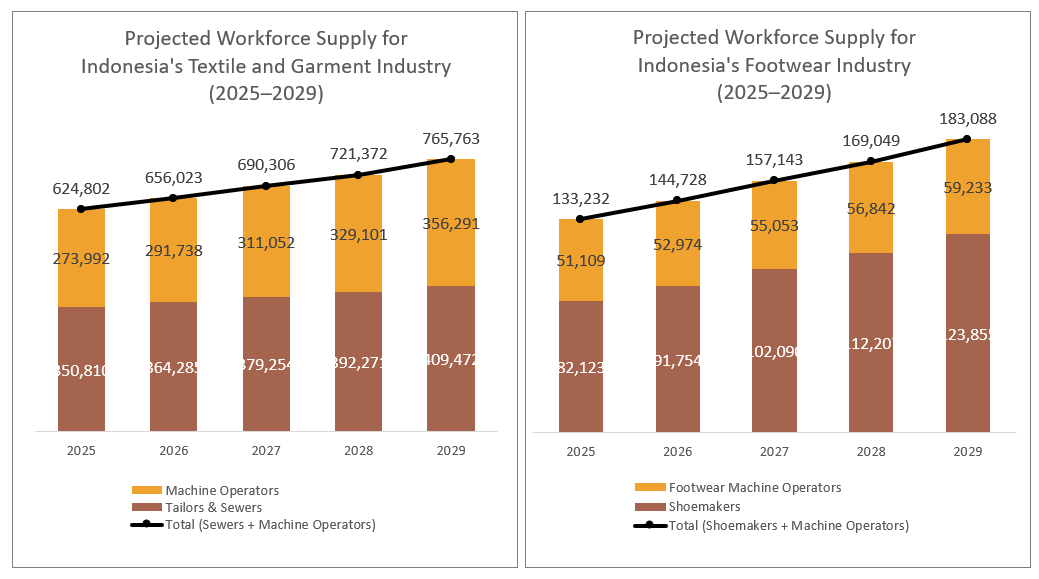
\includegraphics[width=0.95\linewidth,height=\textheight,keepaspectratio]{fig/workforce_projection.png}

}

\caption[\label{fig-workforce}Proyeksi pasokan tenaga kerja untuk
industri tekstil \& garmen, dan alas kaki Indonesia. Sumber: Kementerian Ketenagakerjaan.]{\label{fig-workforce}Proyeksi pasokan tenaga kerja untuk
industri tekstil \& garmen, dan alas kaki Indonesia\footnotemark{}. Sumber: Kementerian Ketenagakerjaan.}

\end{figure}%
\footnotetext{Proyeksi
  Pasokan Tenaga Kerja Lulusan Pendidikan dan Pelatihan Vokasi (SMK dan
  Diploma).}

Jumlah lulusan yang diproyeksikan tersebut jauh melampaui estimasi
permintaan tenaga kerja yang terkait dengan aktivitas investasi terkini.
Data yang dikumpulkan untuk kajian ini menunjukkan bahwa 27 pabrik
tekstil dan alas kaki yang baru berdiri diperkirakan menciptakan
lapangan kerja pada 2025--2026 bagi sekitar 108.000 pekerja.
Dibandingkan dengan aliran lulusan vokasi tahunan yang melampaui 750.000
orang pada 2025, hal ini menunjukkan bahwa ketersediaan tenaga kerja
kecil kemungkinan menjadi kendala mengikat bagi kedua industri dalam
waktu dekat.

Sebaliknya, isu yang lebih penting tampaknya adalah produktivitas dan
kesiapan kerja tenaga kerja. Diskusi dengan pemangku kepentingan
industri menunjukkan adanya perbedaan produktivitas yang substansial
antarlokasi produksi. Manufaktur alas kaki yang beroperasi di klaster
industri mapan di Tangerang, misalnya, melaporkan output per pekerja
yang jauh lebih tinggi dibandingkan fasilitas yang lebih baru di Jawa
Tengah. Data produktivitas yang dibagikan dalam konsultasi menunjukkan
rentang sekitar 1,6 hingga hampir 5,0 pasang sepatu yang diproduksi per
pekerja per hari. Pelaku industri mengaitkan sebagian besar variasi
tersebut dengan perbedaan pengalaman tenaga kerja, kurva belajar pabrik,
kapabilitas penyeliaan, dan kematangan operasional.

Seiring fasilitas yang lebih baru memperoleh pengalaman dan
menyempurnakan proses produksinya, sebagian dari kesenjangan
produktivitas yang teramati semestinya menyempit seiring waktu. Meskipun
demikian, temuan tersebut menegaskan pentingnya kesiapan tenaga kerja
dan pengembangan keterampilan agar pusat-pusat produksi baru mampu
menerjemahkan ketersediaan tenaga kerja menjadi peningkatan
produktivitas seiring investasi yang terus berkembang.

Sebagaimana telah dibahas sebelumnya, posisi Indonesia di dalam rantai
nilai tekstil dan garmen, serta alas kaki terkonsentrasi pada kegiatan
manufaktur dan perakitan. Karena itu, daya saing sangat bergantung pada
efisiensi dan konsistensi produksi, alih-alih pada kapabilitas hulu yang
padat modal atau nilai hilir yang digerakkan merek. Sementara itu, pada
segmen rantai nilai ini, produktivitas tenaga kerja dapat dipengaruhi
secara langsung melalui kebijakan domestik, misalnya melalui reformasi
kurikulum SMK.

Mengingat SMK merupakan jalur utama lulusan vokasi yang memasuki
industri tekstil dan garmen, serta alas kaki, kesenjangan produktivitas
yang teramati memunculkan pertanyaan kebijakan yang penting: apakah
kurikulum vokasi saat ini telah cukup selaras dengan kebutuhan industri
dan lingkungan produksi yang akan dimasuki para lulusan. Hal ini perlu
ditelaah lebih dekat, termasuk sejauh mana jurusan vokasi terkait
tekstil dan garmen berorientasi pada proses produksi industrial berbasis
lini, alih-alih model produksi individual atau bervolume kecil. Yang
patut dicatat, hingga 2026, alas kaki belum merupakan jurusan vokasi
tersendiri di dalam sistem SMK. Alas kaki justru diajarkan sebagai modul
di dalam kurikulum Kriya Kulit dan Imitasi yang lebih luas, meskipun
alas kaki memiliki proses produksi yang khas dan berstatus sebagai
industri berorientasi ekspor yang signifikan.

Menangani keselarasan ini, misalnya melalui kolaborasi yang lebih erat
antara lembaga vokasi dan industri dalam pengembangan kurikulum,
kemungkinan akan diperlukan untuk memastikan bahwa pertumbuhan
kuantitatif pasokan tenaga kerja yang kuat diterjemahkan menjadi tenaga
kerja yang mampu memenuhi standar produktivitas yang dibutuhkan untuk
menjaga daya saing Indonesia dalam rantai nilai tekstil dan garmen,
serta alas kaki global.

\section{Kebijakan Pemerintah dan Program
Dukungan}\label{kebijakan-pemerintah-dan-program-dukungan}

Pemerintah Indonesia telah memperkenalkan beragam kebijakan yang
memengaruhi industri tekstil dan alas kaki, mencakup perdagangan,
investasi, modernisasi permesinan, dan pengembangan tenaga kerja.

Di bidang perdagangan, Permendag No.~17/2025 memperkenalkan persyaratan
impor bagi berbagai produk tekstil, termasuk Persetujuan Impor dan
Laporan Surveyor. Regulasi ini bertujuan memperkuat pengawasan atas
impor tekstil sekaligus menyeimbangkan kebutuhan industri dalam negeri
dan pengguna di hilir. Hal ini ditindaklanjuti dengan Permenperin
No.~27/2025, yang mengatur penerbitan pertimbangan teknis (pertek) untuk
impor tekstil, khususnya guna memastikan ketersediaan bahan baku bagi
kegiatan manufaktur dalam negeri.

Indonesia juga terus memanfaatkan instrumen pemulihan perdagangan
(\emph{trade remedy}) di sektor tekstil, termasuk bea masuk antidumping
(BMAD) dan tindakan pengamanan (BMTP) atas produk-produk tertentu.
Tindakan yang telah berlangsung lama mencakup bea masuk antidumping atas
impor \emph{Polyester Staple Fiber} dari India, Tiongkok, dan Taiwan,
serta \emph{spin drawn yarn} dari Tiongkok. Yang lebih baru, tambahan
tindakan antidumping dan pengamanan telah diterapkan pada produk seperti
kain tenun dari kapas dan benang kapas melalui PMK 48/2024, PMK 67/2025,
dan PMK 98/2025. Tindakan-tindakan tersebut ditujukan untuk menangani
praktik perdagangan tidak adil dan lonjakan impor yang dapat merugikan
produsen dalam negeri. Namun, dampaknya bervariasi antarsegmen industri.
Meskipun tindakan tersebut dapat memberikan perlindungan tambahan bagi
manufaktur domestik yang bersaing langsung dengan impor, tindakan
tersebut juga dapat menaikkan biaya input bagi perusahaan yang bertumpu
pada bahan baku dan barang antara impor.

Pemerintah juga telah memperkenalkan beragam insentif untuk mendorong
investasi di sepanjang rantai nilai tekstil dan alas kaki. Insentif
tersebut meliputi fasilitas bea masuk untuk mesin dan peralatan
berdasarkan PMK 179/2009, insentif perpajakan untuk investasi baru pada
industri padat karya berdasarkan PMK 16/2020, dan fasilitas \emph{tax
holiday} berdasarkan PMK 130/2020 bagi industri pionir yang memenuhi
syarat. Beberapa insentif tersebut juga relevan bagi industri hulu,
termasuk industri kimia dasar, yang berperan penting dalam produksi
serat sintetis dan input tekstil lainnya.

Di bidang pengembangan tenaga kerja, pemerintah telah memperkenalkan
insentif untuk mendukung program pemagangan, pelatihan tenaga kerja, dan
kegiatan penelitian melalui skema \emph{super deduction tax} berdasarkan
PMK 128/2019 dan PMK 153/2020. Dukungan tambahan juga diberikan kepada
industri padat karya, termasuk sektor tekstil dan alas kaki, melalui
fasilitas pajak penghasilan ditanggung pemerintah berdasarkan PMK
10/2025 dan PMK 105/2025.

Untuk mendukung modernisasi permesinan, pemerintah saat ini menjalankan
dua program yang saling melengkapi. Pertama, Program Restrukturisasi
Mesin dan Peralatan (Permenperin 20/2024), yang memberikan penggantian
sebagian atas pembelian mesin dan peralatan produksi baru. Pada program
2026, perusahaan dapat menerima penggantian hingga 25 persen dari nilai
pembelian untuk mesin produksi dalam negeri dan 10 persen untuk mesin
impor, dengan batas maksimum penggantian sebesar Rp500 juta per
perusahaan. Kedua, Program Insentif Reinvestasi Padat Karya (KIPK), yang
memberikan subsidi bunga sebesar 5 persen atas kredit investasi berkisar
Rp500 juta hingga Rp10 miliar. Pemangku kepentingan industri pada
umumnya memandang program-program tersebut sebagai langkah positif untuk
mendukung modernisasi industri, namun mengidentifikasi sejumlah
tantangan implementasi, termasuk plafon penggantian yang relatif
terbatas, tidak tercakupnya peralatan pendukung, dan persyaratan
kelayakan yang dapat membatasi partisipasi.

\subsection{Reformasi Regulasi sebagai Pendorong Daya Saing
Industri}\label{reformasi-regulasi-sebagai-pendorong-daya-saing-industri}

Pencapaian ambisi ekspor tersebut akan bergantung tidak hanya pada
pembiayaan dan insentif, tetapi juga pada kecepatan komitmen investasi
diterjemahkan menjadi pabrik yang beroperasi dan pekerja yang terserap.
Dua area regulasi sangat relevan dalam hal ini: perizinan berusaha dan
pertimbangan teknis impor (pertek impor) bahan baku industri.
Langkah-langkah telah diambil pada kedua bidang tersebut, meskipun
sejauh mana keduanya memenuhi tujuannya akan bergantung pada
implementasi yang konsisten dan terukur di seluruh kementerian/lembaga
dan daerah.

Pertama, pada bidang perizinan berusaha, keterlibatan DEN dengan pelaku
sektor tekstil dan garmen di Jawa Barat, Jawa Tengah, Banten, dan Jawa
Timur mengidentifikasi 27 perusahaan dengan total 108.179 pekerja yang
lini waktu realisasi investasinya sensitif terhadap durasi perizinan
(Gambar~\ref{fig-pipeline}).

\begin{figure}[htbp!]

\centering{

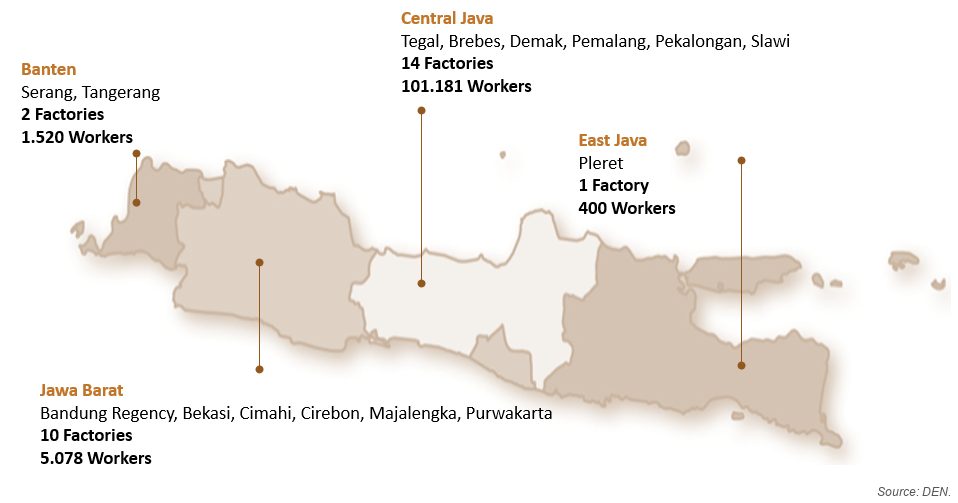
\includegraphics[width=1\linewidth,height=\textheight,keepaspectratio]{fig/investment_pipeline.png}

}

\caption{\label{fig-pipeline}Pipeline investasi tekstil, garmen \& alas
kaki (2025--2026). Sumber: DEN.}

\end{figure}%

Penelaahan lebih dalam atas satu fasilitas alas kaki di Jawa Tengah yang
mempekerjakan 12.000 pekerja mengilustrasikan sejauh mana keterlambatan
perizinan dapat menghambat realisasi investasi. Proses AMDAL (izin
lingkungan) saja memakan waktu sekitar 1.095 hari, yang mencakup
sebagian besar lini waktu perizinan proyek tersebut
(Gambar~\ref{fig-licensing}).

\begin{figure}[htbp!]

\centering{

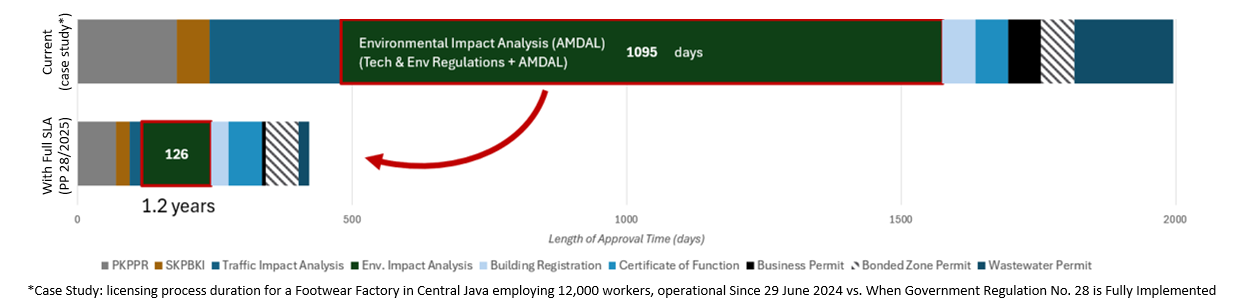
\includegraphics[width=1\linewidth,height=\textheight,keepaspectratio]{fig/licensing_time.png}

}

\caption{\label{fig-licensing}Potensi pengurangan waktu persetujuan
investasi melalui implementasi penuh PP No.~28/2025. Sumber: DEN.}

\end{figure}%

Meskipun kasus ini bersifat ilustratif dan bukan representatif,
tantangan serupa dilaporkan terjadi di seluruh sektor. Peraturan
Pemerintah No.~28 Tahun 2025 berupaya mengatasi hambatan tersebut dengan
memperkenalkan \emph{Service Level Agreement} (SLA) dengan lini waktu
pemrosesan yang jelas untuk setiap tahap persetujuan. Implementasi
penuhnya dapat memangkas total waktu perizinan dari 2--3 tahun menjadi
sekitar 1,2 tahun, termasuk pengurangan waktu pemrosesan AMDAL dari
1.095 hari menjadi 126 hari. Efektivitas reformasi tersebut pada
akhirnya akan bergantung pada penegakan yang konsisten dan koordinasi
yang kuat di seluruh tingkatan pemerintahan.

Kedua, di luar perizinan berusaha, efisiensi proses persetujuan impor
tetap menjadi faktor penting yang memengaruhi realisasi investasi dan
daya saing industri. Dalam konteks ini, Satgas P3-MPPE, yang dibentuk
berdasarkan Keputusan Presiden No.~4 Tahun 2026 dan dikoordinasikan oleh
Kementerian Koordinator Bidang Perekonomian, telah menetapkan
penyederhanaan pertimbangan teknis impor bahan baku industri sebagai
prioritas reformasi awal. Inisiatif ini mencakup penyesuaian persyaratan
pertimbangan teknis di bawah Kementerian Perindustrian serta revisi
kebijakan perdagangan terkait di bawah Kementerian Perdagangan.

Bagi sektor tekstil dan alas kaki, reformasi tersebut sangat relevan.
Manufaktur bertumpu pada akses yang tepat waktu terhadap serat, benang,
bahan kimia, dan input antara terspesialisasi lainnya yang kerap
ditentukan oleh pembeli global dan prinsipal merek. Keterlambatan
memperoleh pertimbangan teknis impor atau mengeluarkan bahan impor dapat
mengganggu jadwal produksi, menaikkan biaya operasional, dan menurunkan
keandalan rantai pasok.

Isu ini menjadi semakin penting seiring Indonesia memperluas kapasitas
tekstil hulunya melalui investasi benang dan kain yang baru.
Fasilitas-fasilitas tersebut akan berperan kritis dalam memungkinkan
pemenuhan persyaratan transformasi ganda IEU-CEPA, sehingga administrasi
impor yang efisien menjadi pelengkap penting bagi upaya pembangunan
industri yang lebih luas.

Secara keseluruhan, reformasi pada perizinan berusaha dan persetujuan
impor menyentuh dua area regulasi yang secara langsung memengaruhi laju
realisasi investasi di sektor tekstil dan alas kaki. Jika
diimplementasikan secara efektif, langkah-langkah tersebut dapat
mempercepat eksekusi proyek, memperkuat kepercayaan investor, dan
mendukung penciptaan lapangan kerja yang lebih cepat. Indonesia telah
memperkenalkan banyak instrumen kebijakan yang diperlukan; tantangan
utamanya kini terletak pada memastikan implementasi yang konsisten di
seluruh institusi dan tingkatan pemerintahan.

\section{Kesimpulan}\label{kesimpulan}

Industri tekstil dan alas kaki Indonesia tetap penting secara strategis,
tidak hanya karena kontribusinya terhadap ekspor, tetapi juga karena
perannya sebagai salah satu sumber lapangan kerja manufaktur formal
terbesar di negara ini. Kedua industri berada pada posisi yang baik
untuk memperoleh manfaat dari sejumlah perkembangan yang menguntungkan,
termasuk diversifikasi pengadaan global menjauh dari Tiongkok,
meningkatnya minat investor terhadap Asia Tenggara, dan penyelesaian
secara substansi \emph{Indonesia--European Union Comprehensive Economic
Partnership Agreement} (IEU-CEPA). Secara bersama-sama, perkembangan
tersebut menciptakan jendela peluang bagi Indonesia untuk memperkuat
posisinya di dalam rantai nilai tekstil dan alas kaki global.

Temuan kajian ini menunjukkan bahwa tantangan daya saing Indonesia pada
dasarnya bukanlah persoalan biaya produksi. Relatif terhadap negara
pesaing utama, Indonesia secara umum masih kompetitif pada biaya tenaga
kerja, energi, dan air. Sebaliknya, kendala yang lebih signifikan
berkaitan dengan realisasi investasi, peningkatan teknologi,
produktivitas tenaga kerja, dan kemampuan memenuhi persyaratan pasar
yang semakin menuntut, khususnya yang terkait keberlanjutan dan
ketertelusuran.

Kajian ini juga menyoroti pentingnya mengenali keragaman struktural
industri ini. Sektor tekstil dan alas kaki Indonesia terdiri atas
manufaktur yang terintegrasi secara global dan terhubung dengan pembeli
internasional, sekaligus produsen berorientasi domestik yang melayani
pasar lokal. Perbedaan juga terdapat di sepanjang rantai nilai itu
sendiri, dengan segmen hulu menghadapi tantangan terkait intensitas
modal, skala, dan ketersediaan bahan baku, sementara segmen hilir lebih
banyak bergantung pada produktivitas tenaga kerja, efisiensi
operasional, dan akses pasar. Akibatnya, intervensi kebijakan perlu
disesuaikan dengan kendala spesifik yang dihadapi segmen yang berbeda,
alih-alih bertumpu pada pendekatan yang seragam.

Dalam jangka pendek, perbaikan kecepatan dan keterprediksian realisasi
investasi semestinya menjadi prioritas kebijakan. Bukti yang dikumpulkan
dalam kajian ini menunjukkan bahwa proses perizinan yang panjang dan
hambatan administratif dapat secara signifikan menunda pembangunan
pabrik dan penciptaan lapangan kerja. Reformasi perizinan berusaha dan
prosedur persetujuan impor yang sedang berjalan karena itu berpotensi
menghasilkan manfaat ekonomi yang substansial dengan mempercepat
implementasi investasi, memperkuat kepercayaan investor, dan mendukung
penciptaan lapangan kerja.

Dalam jangka yang lebih panjang, kemampuan Indonesia menangkap nilai
yang lebih besar dari industri tekstil dan alas kaki akan bergantung
pada penguatan ekosistem industri domestik dan perbaikan produktivitas.
Meskipun proyeksi tenaga kerja menunjukkan bahwa pasokan tenaga kerja
kecil kemungkinan menjadi kendala mengikat, kesenjangan produktivitas
yang signifikan masih terdapat antarlokasi produksi, yang menegaskan
pentingnya kesiapan tenaga kerja, pendidikan vokasi, dan pengembangan
keterampilan yang relevan dengan industri. Pada saat yang sama,
investasi berkelanjutan pada modernisasi permesinan, pemenuhan aspek
keberlanjutan, dan kapabilitas industri hulu akan diperlukan untuk
meningkatkan nilai tambah domestik dan mendukung pemenuhan persyaratan
pasar global yang terus berkembang.

Pada akhirnya, peluang Indonesia bukan sekadar menarik lebih banyak
investasi tekstil dan alas kaki, melainkan memperdalam partisipasinya
dalam rantai nilai global sekaligus meningkatkan nilai domestik yang
tercipta dari partisipasi tersebut. Pencapaian tujuan ini menuntut
pendekatan terkoordinasi yang memadukan reformasi regulasi, peningkatan
industri, pengembangan tenaga kerja, dan pembangunan ekosistem. Jika
tantangan-tantangan tersebut dapat ditangani secara efektif, industri
tekstil dan alas kaki dapat tetap menjadi sumber penting pertumbuhan
ekspor, lapangan kerja formal, dan transformasi industri pada
tahun-tahun mendatang.

\section*{Pernyataan
Reproduktibilitas}\label{pernyataan-reproduktibilitas}
\addcontentsline{toc}{section}{Pernyataan Reproduktibilitas}

Berkas sumber makalah ini tersedia di
\url{https://github.com/imedkrisna/tekstil}. Seluruh gambar berbasis
data (Gambar~\ref{fig-growth}, Gambar~\ref{fig-recovery},
Gambar~\ref{fig-investment}, Gambar~\ref{fig-globalimport},
Gambar~\ref{fig-smile}, Gambar~\ref{fig-trade},
Gambar~\ref{fig-workers}) dihasilkan oleh notebook Jupyter
\texttt{fig/fig.ipynb} dari berkas Excel pada folder \texttt{fig/};
jumlah tenaga kerja Sakernas yang mendasari Gambar~\ref{fig-workers}
dimasukkan langsung di dalam notebook. Pangsa pasar pada
Tabel~\ref{tbl-shares} dihitung pada notebook yang sama dari data
bilateral UN COMTRADE (\texttt{TradeData.xlsx}), yang tidak
didistribusikan ulang di dalam repositori; notebook tersebut menyimpan
output yang telah dihitung. Gambar-gambar lainnya (diagram rantai nilai,
peta, dan grafik berbasis kerja lapangan DEN serta basis data pihak
ketiga) disertakan sebagai gambar statis pada \texttt{fig/}; kedua peta
dipotong dari aslinya, yang disimpan pada folder yang sama dengan
akhiran \texttt{\_original}.

\phantomsection\label{refs}
\begin{CSLReferences}{1}{1}
\bibitem[\citeproctext]{ref-aprayon2024}
Asia Pacific Rayon. 2024. \emph{Sustainability Report 2024: Clean
Manufacturing at the Forefront}. Asia Pacific Rayon.
\url{https://www.aprayon.com/id/keberlanjutan/dasbor-keberlanjutan/}.

\bibitem[\citeproctext]{ref-adb2025mrio}
Asian Development Bank. 2025. \emph{ADB Multiregional Input-Output
Tables at Current Prices}.
\url{https://kidb.adb.org/globalization/current}.

\bibitem[\citeproctext]{ref-bps2025sakernas}
BPS. 2025a. \emph{Booklet Sakernas Februari 2025}. Vol. 8. BPS.
\url{https://www.bps.go.id/id/publication/2025/07/14/90a6b20c25c63176d23ab46c/booklet-sakernas-februari-2025.html}.

\bibitem[\citeproctext]{ref-bps2025tpt}
BPS. 2025b. \emph{Tingkat Pengangguran Terbuka Menurut Provinsi
(Persen), 2024--2025}.
\url{https://www.bps.go.id/id/statistics-table/2/NTQzIzI=/tingkat-pengangguran-terbuka-menurut-provinsi.html}.

\bibitem[\citeproctext]{ref-costa2025dpp}
Costa, Antonio Braz. 2025. \emph{Digital Product Passport Impacts on the
Global Supply Chain and Technology Requirements}. ITMF Annual Conference
\& IAF World Fashion Convention, Yogyakarta.
\url{https://www.itmf-iaf-conference-2025-yogyakarta.org/conference-downloads-25}.

\bibitem[\citeproctext]{ref-deviyana2025}
Deviyana, Nia. 2025. {``19 Ribu Bal Pakaian Bekas Diduga Impor Ilegal
Diamankan, Nilainya Rp112 Miliar.''} \emph{IDXChannel}, 2025.
\url{https://www.idxchannel.com/news/19-ribu-bal-pakaian-bekas-diduga-impor-ilegal-diamankan-nilainya-rp112-miliar}.

\bibitem[\citeproctext]{ref-ec2024espr}
European Commission. 2024. \emph{Ecodesign for Sustainable Products
Regulation}.
\url{https://commission.europa.eu/energy-climate-change-environment/standards-tools-and-labels/products-labelling-rules-and-requirements/ecodesign-sustainable-products-regulation_en}.

\bibitem[\citeproctext]{ref-feenstra2021}
Feenstra, Robert C., dan Alan M. Taylor. 2021. \emph{International
Macroeconomics}. 5 ed. Worth.

\bibitem[\citeproctext]{ref-fernandezstark2011}
Fernandez-Stark, Karina, Stacey Frederick, dan Gary Gereffi. 2011.
\emph{The Apparel Global Value Chain: Economic Upgrading and Workforce
Development}. Center on Globalization, Governance \& Competitiveness.

\bibitem[\citeproctext]{ref-gereffi2010}
Gereffi, Gary, dan Stacey Frederick. 2010. \emph{The Global Apparel
Value Chain, Trade and the Crisis: Challenges and Opportunities for
Developing Countries}. World Bank.
\url{https://doi.org/10.1596/1813-9450-5281}.

\bibitem[\citeproctext]{ref-gereffi2005governance}
Gereffi, Gary, John Humphrey, dan Timothy Sturgeon. 2005. {``The
Governance of Global Value Chains.''} \emph{Review of International
Political Economy} 12 (1): 78--104.

\bibitem[\citeproctext]{ref-goto2023}
Goto, Kenta. 2023. {``Viet Nam's Textile and Garment Industry in the
Global Value Chain.''} Dalam \emph{Viet Nam 2045: Development Issues and
Challenges}. ERIA.
\url{https://www.eria.org/uploads/16_ch_12-Textile-and-Garment-Industry-in-GVC.pdf}.

\bibitem[\citeproctext]{ref-gupta2022gvc}
Gupta, Krisna, Irma Tsuraya Choirinnida, dan Muhammad Taufik. 2022.
{``Global Value Chain Impact for Indonesia Economy and the Way to Make
It More Resilient.''} Dalam \emph{Indonesia Post-Pandemic Outlook:
Rethinking Health and Economics Post-COVID-19}. Sustainable Indonesia.
Penerbit BRIN. \url{https://penerbit.brin.go.id/press/catalog/book/537}.

\bibitem[\citeproctext]{ref-gupta2022neraca}
Gupta, Krisna, Deasy Pane, dan Donny Pasaribu. 2022. {``The Advent of a
New Trade Governance after the Omnibus Law: Neraca Komoditas.''}
\emph{CIPS Policy Paper} 47.
\url{https://www.cips-indonesia.org/publications/the-advent-of-a-new-trade-governance-after-the-omnibus-law\%3A-neraca-komoditas?lang=id}.

\bibitem[\citeproctext]{ref-hasran2025}
Hasran, Krisna Gupta, dan Rasya Athalla Aaron. 2025. {``Dampak Sistem
Neraca Komoditas terhadap Birokrasi Perdagangan dan Harga Pangan di
Indonesia.''} \emph{CIPS Policy Paper} 44.
\url{https://www.cips-indonesia.org/publications/dampak-sistem-neraca-komoditas-terhadap-birokrasi-perdagangan-dan-harga-pangan-di-indonesia?lang=id}.

\bibitem[\citeproctext]{ref-hodrick1997}
Hodrick, Robert J., dan Edward C. Prescott. 1997. {``Postwar U.S.
Business Cycles: An Empirical Investigation.''} \emph{Journal of Money,
Credit and Banking} 29 (1): 1--16.
\url{https://doi.org/10.2307/2953682}.

\bibitem[\citeproctext]{ref-kartasasmita2025}
Kartasasmita, Agus Gumiwang. 2025. \emph{Keynote Speech by the Minister
of Industry}. ITMF Annual Conference \& IAF World Fashion Convention,
Yogyakarta.
\url{https://www.itmf-iaf-conference-2025-yogyakarta.org/conference-downloads-25}.

\bibitem[\citeproctext]{ref-kemenko2025}
Kemenko Perekonomian. 2025. \emph{Pemerintah Tingkatkan Penguatan Akses
Pembiayaan Produktif dengan Kredit Alsintan dan Kredit Industri Padat
Karya}. Siaran Pers HM.02.04/287/SET.M.EKON.3/08/2025.
\url{https://www.ekon.go.id/publikasi/detail/6527/pemerintah-tingkatkan-penguatan-akses-pembiayaan-produktif-dengan-kredit-alsintan-dan-kredit-industri-padat-karya}.

\bibitem[\citeproctext]{ref-kemenkeu2024}
Kementerian Keuangan. 2024. \emph{APBN Kita: Kinerja dan Fakta, Oktober
2024}. Kementerian Keuangan.
\url{https://media.kemenkeu.go.id/getmedia/4924fc3f-9748-4530-8757-dd7a123b4c73/APBN-KiTa-Oktober-2024.pdf?ext=.pdf}.

\bibitem[\citeproctext]{ref-kemenkeu2025}
Kementerian Keuangan. 2025. \emph{Laporan Belanja Perpajakan 2024}.
Kementerian Keuangan.
\url{https://fiskal.kemenkeu.go.id/publikasi/tax-expenditure-report}.

\bibitem[\citeproctext]{ref-kumparan2026}
KumparanBISNIS. 2026. {``Fakta-Fakta Pembentukan BUMN Tekstil dengan
Modal Rp 101 T.''} \emph{Kumparan}, 2026.
\url{https://kumparan.com/kumparanbisnis/fakta-fakta-pembentukan-bumn-tekstil-dengan-modal-rp-101-t-26dtdGAXO6Z/full}.

\bibitem[\citeproctext]{ref-lubis2025}
Lubis, Daniel Bastian. 2025. \emph{Keadaan Ketenagakerjaan Agustus
2025}. Workshop Penyusunan Laporan Tahunan Dewan Ekonomi Nasional,
Bogor.

\bibitem[\citeproctext]{ref-masitoh2024}
Masitoh, Siti. 2024. {``Tekstil Banyak Menikmati Fasilitas Kawasan
Berikat.''} \emph{Kontan}, 2024.
\url{https://insight.kontan.co.id/news/tekstil-banyak-menikmati-fasilitas-kawasan-berikat}.

\bibitem[\citeproctext]{ref-kemenperin2024}
Ministry of Industry. 2024. \emph{Peta Potensi Industri Alas Kaki Skala
Menengah \& Besar di Indonesia 2024}. Balai Pemberdayaan Industri
Persepatuan Indonesia (BPIPI).
\url{https://datacenter-bpipi.kemenperin.go.id/}.

\bibitem[\citeproctext]{ref-kemenperin2025}
Ministry of Industry. 2025. \emph{Arah Program dan Kegiatan Pengembangan
Sektor Industri Tekstil dan Pakaian Jadi Tahun 2026--2029}. Forum
Kebijakan Strategis: {``Bedah Hasil Kajian Arah Pengembangan Industri
Tekstil dan Pakaian Jadi yang Berkelanjutan dan Berdaya Saing Global,''}
Jakarta.

\bibitem[\citeproctext]{ref-ramadhan2025}
Ramadhan, Gaffari. 2025. \emph{Navigating Uncertainty \& Adopting
Technology -- Pathways to Sustainable Strength in the Textile and
Apparel Industry}. ITMF Annual Conference \& IAF World Fashion
Convention, Yogyakarta.
\url{https://www.itmf-iaf-conference-2025-yogyakarta.org/conference-downloads-25}.

\bibitem[\citeproctext]{ref-razzak1997}
Razzak, W. 1997. {``The Hodrick-Prescott Technique: A Smoother versus a
Filter: An Application to New Zealand GDP.''} \emph{Economics Letters}
57 (2): 163--168. \url{https://doi.org/10.1016/S0165-1765(97)00178-X}.

\bibitem[\citeproctext]{ref-setiawan2025}
Setiawan, Verda Nano. 2025. {``Serikat Buruh Ungkap 126.160 Pekerja Kena
PHK per Oktober 2025.''} \emph{CNBC Indonesia}, 2025.
\url{https://www.cnbcindonesia.com/news/20251108133216-4-683454/serikat-buruh-ungkap-126160-pekerja-kena-phk-per-oktober-2025}.

\bibitem[\citeproctext]{ref-yan2025}
Yan, Yan. 2025. \emph{Sustainability-Driven Development: China's Textile
Policy Framework \& Collaborative Action}. ITMF Annual Conference \& IAF
World Fashion Convention, Yogyakarta.
\url{https://www.itmf-iaf-conference-2025-yogyakarta.org/conference-downloads-25}.

\end{CSLReferences}

\end{document}
